% Clase de documento
\documentclass[letterpaper,12pt,oneside]{book}
% Paquetes
\usepackage[utf8]{inputenc}                                           % Codificación de caracteres
\usepackage[T1]{fontenc}                                              % Codificación de salida
\usepackage[spanish,es-nodecimaldot,es-tabla]{babel}                  % Idioma español
\usepackage{graphicx}                                                 % Para insertar imágenes
\usepackage[top=1in, left=0.9in, right=1.25in, bottom=1in]{geometry}  % Márgenes
\usepackage{tikz}                                                     % Para crear gráficos
\usepackage{tocloft}                                                  % Para personalizar la tabla de contenido
\usepackage{setspace}                                                 % Para el interlineado
\usepackage[backend=biber,style=numeric, sorting=none, doi=false, url=false]{biblatex}                    % Para la bibliografía
\usepackage{csquotes}                                                 % Para citas bibliográficas
\usepackage{amsmath}                                                  % Para ecuaciones matemáticas
\usepackage{amsfonts}
\usepackage{amssymb}
\usepackage[version=4]{mhchem}                                        % Para fórmulas químicas, especificando la versión
\usepackage{booktabs}                                                 % Para mejores líneas en tablas
\usepackage{longtable}                                                % Para tablas largas
\usepackage{siunitx}                                                  % Para el comando \SI y manejo de unidades
\usepackage{pdflscape} % Paquete para orientación horizontal
\usepackage{graphicx}  % Necesario para \centering en algunos casos
\usepackage{rotating} % Paquete para el entorno sidewaystable
\usepackage{subcaption}
\usepackage{float}
\DeclareSIUnit\angstrom{\text {Å}}
\graphicspath{{./Imágenes/}}                                          % Ruta de las imágenes

% Archivo de bibliografía
\addbibresource{referencias.bib}

\begin{document}

    
\begin{titlepage}
    \thispagestyle{empty}
    \begin{minipage}[c][0.17\textheight][c]{0.23\textwidth}
        \begin{center}
            
\includegraphics[width=3.5cm, height=3.5cm]{Escudo-UNAM.pdf}
        \end{center}
    \end{minipage}
    \begin{minipage}[c][0.195\textheight][t]{0.725\textwidth}
        \begin{center}
            \vspace{0.3cm}
            \textsc{\large Universidad Nacional Aut\'onoma de M\'exico}\\[0.5cm]
            \vspace{0.3cm}
            \hrule height2.5pt
            \vspace{.2cm}
            \hrule height1pt
            \vspace{.8cm}
            \textsc{Facultad de Química}\\[0.5cm] %
        \end{center}
    \end{minipage}

    \begin{minipage}[c][0.81\textheight][t]{0.20\textwidth}
        \vspace*{5mm}
        \begin{center}
            \hskip2.0mm
            \vrule width1pt height13cm 
            \vspace{5mm}
            \hskip2pt
            \vrule width2.5pt height13cm
            \hskip2mm
            \vrule width1pt height13cm \\
            \vspace{5mm}
            
\includegraphics[height=3.2cm]{logofq.jpeg}
        \end{center}
    \end{minipage}
    \begin{minipage}[c][0.81\textheight][t]{0.75\textwidth}
        \begin{center}
            \vspace{1cm}

            {\large\scshape Estudio de la solvatación del ion Cu\textsuperscript{2+} en agua y metanol mediante dinámica molecular con DFT/M06-2X}\\[.2in]

            \vspace{2cm}            

            \textsc{\LARGE T\hspace{1.5cm}E\hspace{1.5cm}S\hspace{1.5cm}I\hspace{1.5cm}S}\\[0.5cm]
            \textsc{\large que para obtener el t\'itulo de:}\\[0.5cm]
            \textsc{\large Ingeniero Químico}\\[0.5cm]
            \textsc{\large presenta:}\\[0.5cm]
            \textsc{\large {Jorge Angel Rosas Martínez}}\\[2cm]          

            \vspace{0.5cm}

            {\large\scshape Tutores:\\[0.3cm] {Dr. César Iván León Pimentel}}\\[.2in]

            \vspace{0.5cm}

            \large{Ciudad Universitaria, CDMX}{ }{2025}
        \end{center}
    \end{minipage}
\end{titlepage}


    \frontmatter % Páginas preliminares

        \chapter*{Dedicatoria}
\begin{flushright}
  \emph{Dedicatoria ...} \\
  Hola, soy la dedicatoria.
\end{flushright}
\addcontentsline{toc}{chapter}{Dedicatoria}
\thispagestyle{empty}

        \chapter{Agradecimientos}
En este capitulo escribiré los agradecimientos
\spacing{1.5}%\doublespacing
    
        \tableofcontents
        \listoffigures

    \mainmatter % Páginas principales
        \chapter{Introducción}

El catión Cobre(II), \ce{Cu^{2+}}, participa en una amplia y diversa gama de fenómenos, abarcando desde procesos biológicos esenciales hasta complejas interacciones químicas y aplicaciones tecnológicas de vanguardia. Su particular configuración electrónica $d^9$ le confiere propiedades estructurales y redox únicas, convirtiéndolo en un ion con propiedades estructurales y redox únicas, que han sido objeto de numerosos estudios teóricos y experimentales.

\subsection*{Implicaciones en Sistemas Biológicos y la Salud Humana}

En el dominio de la bioquímica, el \ce{Cu^{2+}} es un micronutriente vital. Su función más prominente es como componente clave de numerosas metaloenzimas que catalizan procesos críticos, tales como el transporte de electrones y oxígeno —ejemplificado por la hemocianina— y la oxidación catalítica de sustratos orgánicos como fenoles y aminas \cite{Cu-2014-01, Wa-2024-03, Wa-2017-01, Wa-2009-01}. Adicionalmente, es fundamental para la movilización del hierro durante la síntesis de hemoglobina.

No obstante, la homeostasis del cobre es delicada. Desequilibrios en su concentración están directamente implicados en patologías graves. La regulación deficiente del cobre se ha conectado con trastornos neurodegenerativos como las enfermedades de Parkinson y Alzheimer \cite{Cu-2014-02,Cu-2011-02, Cu-2012-01}. Asimismo, los desequilibrios en los niveles de ceruloplasmina, que facilita el transporte de Cu2+ en el torrente sanguíneo, pueden provocar el síndrome de Menkes o la enfermedad de Wilson \cite{Cu-2001-01, Cu-2017-01}.

\subsection*{Aplicaciones en Catálisis}

Más allá de su rol biológico, los complejos de cobre son herramientas poderosas en la síntesis química y la tecnología. En el campo de la catálisis, son ampliamente utilizados para la construcción de enlaces carbono-carbono y carbono-heteroátomo, y son indispensables en reacciones como el acoplamiento de Sonogashira-Hagihara y la activación de enlaces C-H. El objetivo actual se centra en el desarrollo de catalizadores basados en cobre que no solo sean eficientes y selectivos, sino también respetuosos con el medio ambiente \cite{Cu-2014-01}.

\section{La Química de Coordinación Única del \ce{Cu^{2+}}: El Efecto Jahn-Teller}

La versatilidad fisicoquímica del catión cobre(II) (\ce{Cu^{2+}}) emana directamente de su estructura electrónica \ce{[Ar]}$d^9$ , siendo el fenómeno central que gobierna su comportamiento la distorsión de Jahn-Teller (JTE). Este efecto se manifiesta como una deformación geométrica espontánea que ocurre en moléculas no lineales con un estado electrónico fundamental degenerado. El teorema postula que el sistema reduce su simetría para eliminar dicha degeneración, lo que resulta en una disminución de su energía total \cite{Cu-2019-01}.

En un complejo octaédrico de \ce{Cu^{2+}}, la configuración \ce{[Ar]}$d^9$ presenta orbitales $e_g$ degenerados. La distorsión para resolver esta degeneración emerge de la diferencia en la densidad electrónica entre el metal y los ligandos  y puede presentarse de dos maneras:
\begin{itemize}
    \item \textbf{Elongación (z-out):} Los dos enlaces axiales se alargan y los cuatro ecuatoriales se acortan. Esto ocurre cuando la densidad electrónica es mayor en el eje $z$ y el orbital molecular semiocupado (SOMO por sus siglas en inglés) es el $d_{x^2-y^2}$.
    \item \textbf{Compresión (z-in):} Los cuatro enlaces ecuatoriales se alargan y los dos axiales se acortan. Sucede cuando la densidad electrónica es mayor en el plano $xy$ y el SOMO es el $d_{z^2}$.
\end{itemize}


\begin{figure}[H]
    \centering
    
    % Fila superior: Distorsión z-out (Elongación)
    \begin{subfigure}{0.2\textwidth}
        \centering
        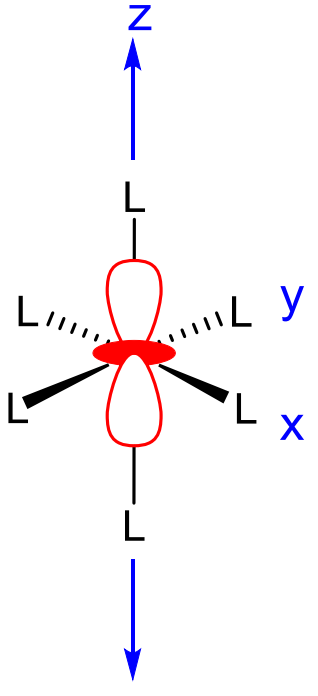
\includegraphics[width=0.5\linewidth]{Imágenes/JTE-z-out-draw.png}
        \caption{}
    \end{subfigure}
    %\hfill % Espacio horizontal entre imágenes
    \begin{subfigure}{0.2\textwidth}
        \centering
        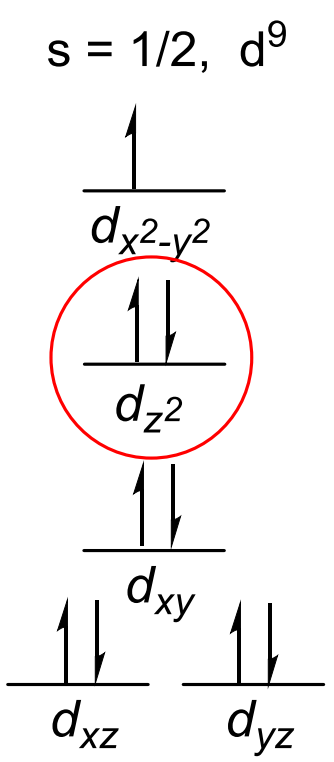
\includegraphics[width=0.5\linewidth]{Imágenes/JTE-z-out-orbitals.png}
        \caption{}
    \end{subfigure}
    
    \vspace{0.5cm} % Espacio vertical entre filas
    
    % Fila inferior: Distorsión z-in (Compresión)
    \begin{subfigure}{0.3\textwidth}
        \centering
        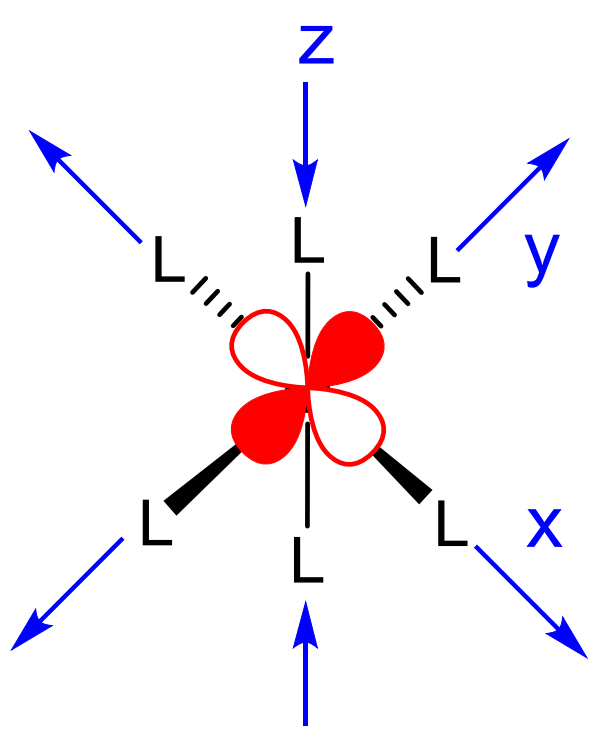
\includegraphics[width=0.5\linewidth]{Imágenes/JTE-z-in-draw.png}
        \caption{}
    \end{subfigure}
    %\hfill % Espacio horizontal entre imágenes
    \begin{subfigure}{0.2\textwidth}
        \centering
        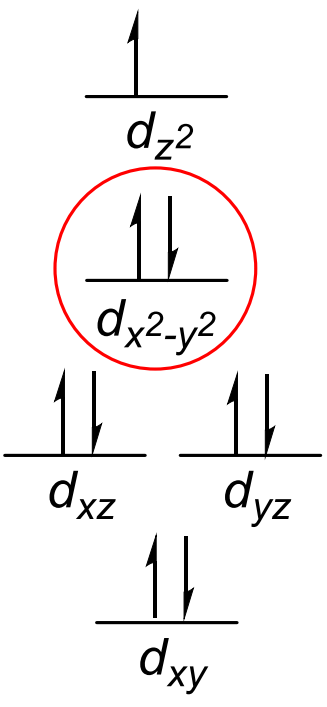
\includegraphics[width=0.5\linewidth]{Imágenes/JTE-z-in-orbitals.png}
        \caption{}
    \end{subfigure}
    
    \caption{Ilustración  del efecto Jahn-Teller de \cite{Cu-2019-01} para un complejo octaédrico del ion Cu(II) con configuración electrónica $d^9$. Arriba se muestra la distorsión por elongación axial (z-out), donde los enlaces axiales se alargan, y su correspondiente desdoblamiento de orbitales. Abajo se presenta la distorsión por compresión axial (z-in), con el acortamiento de los enlaces axiales y su respectivo desdoblamiento energético. La distorsión z-out es la observada más comúnmente en la experimentación .}
    \label{fig:jahn_teller_cu2}
\end{figure}


Aunque la elongación es la geometría más común, estudios teóricos han demostrado que ambas son posibles para el catión \ce{[Cu(OH2)6]^{2+}} \cite{Cu-2019-01}.

El JTE no es un mero detalle, sino la causa directa de la química de coordinación excepcionalmente flexible y dinámica del \ce{Cu^{2+}}. Dota al ion de una plasticidad estructural inusual, permitiéndole adoptar múltiples geometrías (octaédrica distorsionada, piramidal cuadrada, planar cuadrada) con diferencias energéticas muy pequeñas entre ellas. Esta flexibilidad es inherentemente dinámica; en solución, el complejo interconvierte rápidamente entre estas configuraciones. Esto explica la alta labilidad de sus ligandos, cuya tasa de intercambio es órdenes de magnitud superior a la de otros cationes divalentes. La debilidad de los enlaces axiales facilita este rápido intercambio y ha generado un prolongado debate sobre el número de coordinación preferido (4, 5 o 6) del ion en solución.

\section{Hidratación}

\subsection*{Estudios Experimentales}

Históricamente, los estudios experimentales han sido la piedra angular en la comprensión de la solvatación del Cu\textsuperscript{2+}. Las técnicas más utilizadas incluyen:
\begin{itemize}
    \item Difracción de Rayos X y Neutrones
    \item Espectroscopia de Absorción de Rayos X (EXAFS y XANES)
\end{itemize}

Los primeros trabajos de difracción en las décadas de 1970 y 1980 establecieron la idea de una coordinación octaédrica distorsionada (NC=6), con una configuración (4+2) que implicaba cuatro ligandos de agua en posiciones ecuatoriales y dos más distantes en posiciones axiales. Sin embargo, a partir del año 2000, estudios más avanzados, que combinaban técnicas como la difracción de neutrones con dinámica molecular o empleaban análisis de EXAFS y XANES más sofisticados, comenzaron a favorecer un modelo de **coordinación quíntuple (NC=5)** con una geometría de pirámide cuadrada.

Actualmente, existe un consenso experimental sobre las distancias de enlace ecuatoriales ($Cu-O_{eq}$), que se reportan consistentemente en el rango de **1.93--2.00 \AA**. Por el contrario, las distancias axiales ($Cu-O_{ax}$) son más difíciles de medir y presentan una mayor variabilidad, con valores que oscilan entre **2.15 \AA \ y 2.60 \AA**. Investigaciones recientes de alta resolución sugieren incluso la existencia de dos distancias axiales distintas, lo que apunta a un octaedro no centrosimétrico. Algunos estudios que emplean un enfoque multitécnica han llegado a proponer un NC promedio de 4.5, lo que refuerza la idea de una mezcla dinámica de geometrías en solución. La imagen moderna, por tanto, describe una "plasticidad estructural" donde múltiples estados de coordinación coexisten en un equilibrio dinámico.

\subsection*{Estudios Teóricos}

Los estudios computacionales han sido fundamentales para interpretar la evidencia experimental y proporcionar una visión dinámica del proceso de solvatación. Los principales métodos teóricos empleados son:
\begin{itemize}
    \item Teoría del Funcional de la Densidad (DFT)
    \item Dinámica Molecular (MD), tanto clásica como \textit{ab initio} (AIMD)
    \item Métodos híbridos de Mecánica Cuántica/Mecánica Molecular (QM/MM)
\end{itemize}

Las simulaciones teóricas corroboran la naturaleza dinámica del efecto Jahn-Teller, mostrando transformaciones rápidas entre diferentes configuraciones en escalas de tiempo de femtosegundos. Gran parte de los modelos teóricos indican que la geometría de **pirámide cuadrada (NC=5)** es la más estable en solución acuosa, aunque la diferencia de energía con la forma **hexa-coordinada (NC=6)** es muy pequeña ($\sim$1.4 kcal/mol). Esto sugiere que ambas especies pueden coexistir en solución, lo cual está en línea con los hallazgos experimentales más recientes.

Un aporte crucial de los estudios teóricos ha sido resaltar el papel de la segunda capa de solvatación. Se ha demostrado que la formación de enlaces de hidrógeno entre las moléculas de agua de la primera y segunda esfera de hidratación es un factor de estabilización que puede competir energéticamente con la coordinación de una molécula de agua en la posición axial. Las distancias de enlace calculadas concuerdan bien con los datos experimentales, con valores promedio para $Cu-O_{eq}$ de alrededor de **2.00--2.03 \AA** y para $Cu-O_{ax}$ de **2.15--2.30 \AA**. En general, la modelización teórica apoya la visión de un sistema flexible donde coexisten dinámicamente estructuras con NC=5 y NC=6, y descarta una relevancia significativa de la coordinación tetraédrica (NC=4) en el ion Cu\textsuperscript{2+} solvatado en agua.

\section{Solvatación  en Metanol}


Al igual que en el agua, la estructura de solvatación del ion Cu\textsuperscript{2+} en metanol es un área de investigación activa, aunque la cantidad de estudios disponibles es notablemente más escasa. Persiste un debate sobre el número de coordinación (NC) y la geometría predominantes, con diferentes estudios experimentales y teóricos llegando a conclusiones contradictorias. La naturaleza dinámica del ion y la sutil influencia del disolvente complican la obtención de un consenso definitivo. Un resumen detallado de los trabajos más relevantes se encuentra en la Tabla \ref{tab:metanol_corrected}.

\subsection*{Estudios Experimentales}

Las investigaciones experimentales han empleado diversas técnicas espectroscópicas para determinar la estructura local del Cu\textsuperscript{2+} en metanol. Entre los métodos más destacados se encuentran:
\begin{itemize}
    \item Espectroscopia de absorción de rayos X (EXAFS y XANES)
    \item Análisis de modulación de eco de espín de electrones
    \item Estudios de Resonancia Magnética Nuclear (RMN) de Oxígeno-17
\end{itemize}

El panorama experimental se caracteriza por una falta de acuerdo. Mientras que estudios tempranos (Ichikawa y Kevan, 1980) propusieron una coordinación de \textbf{seis (NC=6)}, trabajos posteriores sugirieron que la técnica empleada podría haber sobrestimado las distancias de enlace. Más tarde, estudios de RMN (Helm et al., 1986) observaron una "rápida transición" de isómeros hexacoordinados a conformaciones de \textbf{cinco coordinaciones (NC=5)}, introduciendo la idea de un equilibrio dinámico.

Este debate continúa en estudios más recientes. Por un lado, Zitolo et al. (2012), combinando EXAFS y XANES, concluyeron "inequívocamente" que el Cu\textsuperscript{2+} en metanol adopta una geometría de \textbf{pirámide cuadrada con NC=5}. Por otro lado, un estudio más reciente de Persson et al. (2020) con EXAFS de alta calidad determinó que el mejor modelo de ajuste correspondía a una estructura \textbf{octaédrica distorsionada por Jahn-Teller con NC=6} y carácter no centrosimétrico, contradiciendo directamente la conclusión anterior.

A pesar de la discrepancia en el NC, hay un mayor consenso en las distancias de enlace ecuatoriales ($Cu-O_{eq}$), reportadas consistentemente en el rango de \textbf{1.95--1.98 \AA}. Las distancias axiales ($Cu-O_{ax}$), sin embargo, varían más, con valores reportados de \textbf{2.23 \AA} para el modelo de NC=5 y dos distancias distintas de aproximadamente \textbf{2.20 \AA \ y 2.34 \AA} para el modelo de NC=6.

\subsection*{Estudios Teóricos}

Los métodos computacionales han sido cruciales para explorar el complejo panorama energético de la solvatación del Cu\textsuperscript{2+} en metanol. Las principales técnicas utilizadas incluyen:
\begin{itemize}
    \item Métodos \textit{ab initio} como MP2
    \item Teoría del Funcional de la Densidad (DFT), en particular con el funcional M06-2X
    \item Modelos de disolvente continuo implícito (IEF-PCM)
\end{itemize}

Los estudios teóricos, principalmente los trabajos exhaustivos de Da-yang et al., han demostrado que el NC más estable depende fuertemente de las condiciones del modelo, como el tamaño del clúster de solvente (n), la temperatura y el entorno (fase gaseosa vs. disolvente implícito).

En la \textbf{fase gaseosa}, los cálculos muestran una competencia entre diferentes números de coordinación. El método MP2 tiende a favorecer isómeros \textbf{tetra- y pentacoordinados}, mientras que el método DFT (M06-2X) favorece a los \textbf{penta- y hexacoordinados}. Para clústeres pequeños (n=1-5), las coordinaciones más bajas son las más estables, pero a medida que aumenta el tamaño, las estructuras de mayor NC ganan relevancia.

La inclusión de un \textbf{modelo de disolvente implícito} (IEF-PCM) tiene un "impacto discernible" y cambia drásticamente el panorama. En este entorno, se observa una clara preferencia por los números de coordinación más altos, desfavoreciendo a las estructuras de NC=4. Para clústeres de mayor tamaño (n=7-10), las estructuras \textbf{hexacoordinadas (NC=6)} dominan "exclusivamente" la población a cualquier temperatura. Este hallazgo subraya la importancia crítica del efecto del medio dieléctrico para estabilizar geometrías más compactas y con mayor número de coordinación.

Las distancias de enlace calculadas teóricamente muestran una "excelente concordancia" con los datos experimentales, con valores de $Cu-O_{eq}$ que oscilan entre \textbf{1.94--2.02 \AA} y de $Cu-O_{ax}$ entre \textbf{2.15--2.27 \AA}. Los cálculos también revelan que el disolvente alarga los enlaces dativos axiales en las estructuras pentacoordinadas en comparación con la fase gaseosa.



\section{Justificación y Enfoque Metodológico}

Históricamente, los métodos experimentales como la difracción de rayos X y neutrones o las espectroscopias EXAFS y XANES han sido cruciales para sondear estos sistemas. Sin embargo, a pesar de su capacidad para medir distancias de enlace con precisión, estos métodos enfrentan limitaciones significativas. A menudo existe una considerable controversia y ambigüedad en la determinación del número de coordinación (NC) y la geometría, y resulta técnicamente difícil distinguir entre estructuras con energías muy similares, como las de coordinación cuádruple, quíntuple y séxtuple, que pueden coexistir en solución.

Frente a estas limitaciones, los métodos teóricos y las simulaciones computacionales emergen como una herramienta indispensable y complementaria. Enfoques como la Dinámica Molecular (MD) basada en la Teoría del Funcional de la Densidad (DFT) permiten superar las desventajas experimentales al proporcionar una visión detallada a nivel atómico. Estos métodos posibilitan la exploración de superficies de energía potencial, la caracterización de efectos dinámicos como la inversión del eje de Jahn-Teller en escalas de tiempo de picosegundos, y el estudio de interacciones complejas como la transferencia de carga y los enlaces de hidrógeno, que son difíciles de aislar experimentalmente. Si bien los métodos teóricos no están exentos de desventajas, como el alto costo computacional y una fuerte sensibilidad a la elección del funcional y la base de conjunto, su capacidad para modelar la dinámica y la coexistencia de múltiples estados los convierte en una opción poderosa para resolver las controversias existentes.

El presente trabajo de tesis aprovecha las ventajas de los métodos teóricos para abordar dos frentes. Primero, se enfoca en la solvatación del Cu\textsuperscript{2+} en metanol, un área donde la información experimental y teórica es notablemente más escasa en comparación con el agua. Este vacío de conocimiento representa un área de oportunidad significativa. Por ello, este trabajo presenta por primera vez en la literatura un estudio teórico exhaustivo sobre la estructura y dinámica de los clústeres de Cu\textsuperscript{2+}(MeOH)\textsubscript{n} utilizando DFT. Segundo, se reexamina el caso del agua. Aunque es un sistema mucho más estudiado, la controversia sobre la predominancia de una coordinación quíntuple o séxtuple persiste. El enfoque teórico permite analizar la coexistencia dinámica de estas especies, ofreciendo una perspectiva que las mediciones experimentales, a menudo promediadas en el tiempo, no pueden capturar completamente.

Para llevar a cabo estos estudios, se ha seleccionado el funcional \textbf{M06-2X}. Esta elección se justifica brevemente aquí, y se detallará a profundidad en capítulos posteriores. El M06-2X se presenta como una alternativa computacionalmente eficiente a métodos \textit{ab initio} más costosos como el MP2, y ha demostrado una excelente concordancia con datos experimentales y teóricos para la descripción de los clústeres de Cu\textsuperscript{2+} en metanol, reproduciendo con precisión las distancias de enlace y las reglas de estabilidad.

En los siguientes capítulos se expondrá el marco teórico detallado de la Dinámica Molecular y la Teoría del Funcional de la Densidad, explicando la naturaleza del funcional M06-2X. Posteriormente, se presentará la metodología computacional empleada para la construcción y simulación de los sistemas en ambos disolventes. Finalmente, se realizará un análisis exhaustivo de los resultados y se presentarán las conclusiones derivadas de este estudio computacional.

        \chapter{Fundamentos de Dinámica Molecular}

\section{Introducción}

\subsection{Modelado y Simulación Molecular}

El objetivo fundamental de la modelización y simulación molecular en la química y la física es el de estudiar la materia a escala atomística \cite[xxv]{zhou2022molecular}. Estas técnicas computacionales se han consolidado como una herramienta potente y esencial en la investigación científica moderna, complementando la interacción tradicional entre la teoría y la experimentación \cite[1]{zhou2022molecular}. La simulación proporciona información detallada sobre las interacciones y los movimientos de los átomos o moléculas constituyentes de un sistema, lo que a su vez permite la predicción y comprensión de sus propiedades macroscópicas \cite[xxv]{zhou2022molecular}.

Para lograrlo, se emplea un modelo definido con precisión que representa el material de interés. Este modelo es, en realidad, una composición de dos aspectos: uno que describe las interacciones entre las moléculas que conforman el sistema y otro que modela las interacciones entre dichas moléculas y su entorno \cite[26]{haile1992molecular}.

\subsection{Limitaciones de los Métodos Experimentales}

El uso de la simulación computacional se justifica por las limitaciones intrínsecas de los métodos puramente experimentales. Frecuentemente, los experimentos se ven restringidos por altos costos, la inaccesibilidad de ciertas condiciones experimentales y las limitaciones del propio equipo de medición \cite[1]{zhou2022molecular}.

Desde una perspectiva fundamental, para realizar una medición experimental, es ineludible que un observador interactúe con el sistema; algún tipo de sonda debe cruzar los límites del sistema para obtener datos. Esto implica que los sistemas verdaderamente aislados no pueden ser estudiados experimentalmente, ya que la propia medición altera su condición de aislamiento. En contraste, las simulaciones moleculares, al ser una forma de teoría, no involucran mediciones en sistemas reales y, por lo tanto, pueden realizar cálculos sobre sistemas verdaderamente aislados y obtener resultados significativos \cite[22]{haile1992molecular}. De esta manera, la simulación actúa como una alternativa al reduccionismo y como una herramienta para poner a prueba teorías \cite[24]{haile1992molecular}.

\subsection{El Puente entre Escalas: De lo Microscópico a lo Macroscópico}

La simulación molecular establece un puente conceptual entre la teoría microscópica y las propiedades macroscópicas observables. Este vínculo se fundamenta en la mecánica estadística, que permite relacionar la información microscópica detallada —como las coordenadas y los momentos de todas las partículas obtenidas durante una simulación— con las propiedades observables de un sistema macroscópico \cite[125]{frenkel2002understanding}.

En una medición física, se registra cómo una sonda (por ejemplo, un termómetro o un manómetro) responde al contacto con el sistema. En cambio, en una simulación, se deduce el valor de estas propiedades a partir del conocimiento completo del estado microscópico \cite[125]{frenkel2002understanding}. La ventaja crucial de la simulación es su capacidad para expandir el horizonte de la complejidad que separa los problemas "resolubles" de los "irresolubles" \cite[3]{MD-2001-01}. Las teorías físicas fundamentales, como la mecánica cuántica o clásica, conducen a ecuaciones que no pueden resolverse analíticamente para sistemas de más de dos cuerpos, un dilema conocido como el problema de los muchos cuerpos (\textit{many-body problem}). La simulación ofrece una vía para abordar numéricamente esta complejidad \cite[3]{MD-2001-01}.

\subsection{Métodos de Simulación Molecular}

Existen dos enfoques numéricos principales para calcular las propiedades observables de sistemas clásicos de muchos cuerpos: los métodos determinísticos, como la Dinámica Molecular (DM), y los métodos estocásticos, como el Monte Carlo (MC).

\subsubsection{Métodos Determinísticos}
Los métodos determinísticos, cuyo principal exponente es la Dinámica Molecular (DM), se basan en la resolución numérica de las ecuaciones de movimiento, típicamente las ecuaciones de Newton \cite[28]{haile1992molecular}. Este procedimiento genera una trayectoria en el espacio de fases ($r^N(t), p^N(t)$), donde las posiciones de las partículas están conectadas en el tiempo, revelando la dinámica del sistema de manera análoga a una película \cite[28, 53]{haile1992molecular}{frenkel2002understanding}.

\subsubsection{Métodos Estocásticos}
Los métodos estocásticos, como el Monte Carlo, no generan trayectorias temporalmente conectadas. En su lugar, las posiciones de las moléculas se generan de manera probabilística, de tal forma que una nueva configuración depende únicamente de la configuración inmediatamente anterior, siguiendo una secuencia conocida como cadena de Markov \cite[28]{haile1992molecular}. Estos métodos están diseñados para evaluar integrales multidimensionales que, en este contexto, corresponden a los promedios de ensamble de la mecánica estadística para propiedades configuracionales \cite[29]{haile1992molecular}.

\subsubsection{Diferencia Conceptual entre Dinámica Molecular y Monte Carlo}
La diferencia clave entre la DM y el MC radica en cómo exploran el espacio de fases de un sistema.

La \textbf{Dinámica Molecular} genera una trayectoria físicamente realista al seguir las leyes del movimiento, proporcionando información tanto de propiedades estáticas como dinámicas (por ejemplo, coeficientes de transporte) \cite[97, 54]{frenkel2002understanding}. Su principal fortaleza es también su mayor debilidad: debe seguir la dinámica natural del sistema, lo que puede ser computacionalmente prohibitivo si los procesos de interés ocurren en escalas de tiempo muy largas \cite[54]{frenkel2002understanding}.

Por otro lado, el \textbf{Monte Carlo} es un método estocástico que no proporciona información sobre la evolución temporal del sistema y, por lo tanto, no puede usarse para calcular propiedades dinámicas \cite[54]{frenkel2002understanding}. Su gran ventaja reside en su flexibilidad para realizar "movimientos de prueba" no físicos, es decir, cambios en la configuración del sistema que no ocurrirían en la naturaleza pero que son cruciales para una equilibración eficiente. Esto es especialmente útil en sistemas donde la dinámica natural es demasiado lenta para ser muestreada adecuadamente con DM, o en simulaciones que requieren intercambio de partículas entre reservorios \cite[405]{frenkel2002understanding}.

\subsection{Fundamentos de la Dinámica Molecular Clásica}

La Dinámica Molecular (DM) es una técnica de simulación computacional utilizada para estudiar sistemas complejos a nivel atómico, siguiendo su evolución temporal para derivar propiedades cinéticas y termodinámicas \cite[2]{MD-2001-01}. En su formulación clásica, la DM trata a las moléculas como objetos clásicos, donde los átomos son esferas y los enlaces actúan como resortes elásticos, y su dinámica está regida por las leyes de la mecánica clásica \cite[2]{MD-2001-01}. El procedimiento consiste en resolver numéricamente las ecuaciones de movimiento de Newton para un sistema de $N$ partículas hasta que sus propiedades se estabilizan (equilibración), para luego realizar mediciones promediadas en el tiempo \cite[97]{frenkel2002understanding}.

La base teórica de la DM es multidisciplinaria e integra conceptos de mecánica clásica, mecánica molecular y mecánica estadística \cite[xxv]{zhou2022molecular}.

\subsubsection{Campos de Fuerza Clásicos y su Parametrización}
En la DM clásica, las interacciones entre partículas se describen mediante una función de energía potencial, $U(r^N)$, comúnmente conocida como campo de fuerza (\textit{force field}). Este campo de fuerza es una descripción aproximada de la superficie de energía potencial real del sistema \cite[53]{frenkel2002understanding}. Su parametrización implica definir formas matemáticas funcionales para los diferentes términos de energía (enlaces, ángulos, torsiones, interacciones no enlazadas) y ajustar los parámetros numéricos de estas funciones.

Para realizar un cálculo, el usuario debe especificar los tipos de átomos presentes, su conectividad (enlaces) y una geometría inicial \cite[69]{jensen2017introduction}. La calidad de una simulación depende críticamente de la precisión del campo de fuerza utilizado, y es importante reconocer que existen diferentes "sabores" o versiones de un mismo campo de fuerza, que varían según su implementación y conjunto de parámetros \cite[69]{jensen2017introduction}.

\subsubsection{Limitaciones de los Campos de Fuerza Clásicos}
El enfoque clásico es una aproximación excelente para el movimiento traslacional y rotacional de una amplia gama de moléculas \cite[97]{frenkel2002understanding}. Sin embargo, su validez disminuye en ciertas situaciones donde los efectos cuánticos son dominantes. Un tratamiento cuántico se vuelve necesario en los siguientes casos:
\begin{itemize}
    \item Para describir el movimiento de átomos muy ligeros, como el helio (He) o el hidrógeno (H$_2$) \cite[97]{frenkel2002understanding}.
    \item Para modelar movimientos vibracionales de alta frecuencia $\nu$, donde la energía del cuanto vibracional es comparable o mayor que la energía térmica, es decir, cuando $h\nu > k_B T$ \cite[97]{frenkel2002understanding}.
    \item Para estudiar procesos que involucran la ruptura y formación de enlaces químicos, ya que los campos de fuerza clásicos asumen una conectividad atómica predefinida y estática, lo cual los incapacita para describir reacciones químicas \cite[R1299]{MD-2002-01}.
\end{itemize}

\subsection{Dinámica Molecular \textit{Ab Initio} (AIMD)}

Para superar las limitaciones de los campos de fuerza, se desarrolló la Dinámica Molecular \textit{Ab Initio} (AIMD). En este enfoque, las fuerzas que actúan sobre los núcleos se calculan "sobre la marcha" (\textit{on the fly}) a partir de cálculos de estructura electrónica, en lugar de utilizar un campo de fuerza empírico \cite[R1297]{MD-2002-01}.

\begin{itemize}
    \item \textbf{Ventajas:} Al tratar explícitamente la estructura electrónica, la AIMD puede describir con precisión fuerzas de muchos cuerpos, polarización electrónica y, fundamentalmente, la ruptura y formación de enlaces químicos. Su precisión está limitada únicamente por la exactitud del método de estructura electrónica empleado \cite[R1299]{MD-2002-01}.
    \item \textbf{Desventajas:} El costo computacional es significativamente mayor que el de la DM clásica. Esto restringe las simulaciones de AIMD a sistemas mucho más pequeños (del orden de decenas o cientos de átomos) y a escalas de tiempo más cortas (del orden de picosegundos) \cite[R1299]{MD-2002-01}.
\end{itemize}

\subsubsection{La Aproximación de Born-Oppenheimer}
La implementación práctica de la AIMD se sustenta en la \textbf{aproximación de Born-Oppenheimer (BO)}, un pilar de la química cuántica \cite[58]{szabo1996modern}. Esta aproximación se basa en la gran diferencia de masa entre los electrones ($m_e$) y los núcleos ($m_N$), donde $m_e/m_N \ll 1$ \cite[58,213]{szabo1996modern}{allen2012computer}.

Dado que los núcleos son mucho más pesados, se mueven de forma mucho más lenta que los electrones. La aproximación BO permite desacoplar el movimiento de ambas partículas, asumiendo que los electrones se mueven en el campo de núcleos fijos o "congelados" \cite[58]{szabo1996modern}. En la práctica, esto significa que para una configuración nuclear dada, se resuelve la ecuación de Schrödinger para los electrones para obtener su energía de estado fundamental. Esta energía electrónica se convierte entonces en la energía potencial que gobierna el movimiento clásico de los núcleos, creando lo que se conoce como la \textit{superficie de energía potencial de Born-Oppenheimer} \cite[213]{allen2012computer}. Esta separación es fundamental, ya que permite calcular las fuerzas sobre los núcleos en cada paso de una trayectoria de DM, a partir de un tratamiento cuántico de los electrones \cite[R1300]{MD-2002-01}.

\subsubsection{BOMD vs. CPMD}
Dentro de la AIMD, existen dos implementaciones principales que difieren conceptualmente en cómo manejan la dinámica del sistema:

\begin{itemize}
    \item \textbf{Dinámica Molecular de Born-Oppenheimer (BOMD):} En este método, se sigue estrictamente la aproximación BO. En cada paso temporal de la dinámica nuclear, se resuelve por completo el problema de la estructura electrónica, es decir, la función de onda electrónica se optimiza hasta converger al estado fundamental para esa geometría nuclear fija. A partir de esta función de onda convergida, se calculan las fuerzas sobre los núcleos \cite[125]{canuto2010solvation}. Aunque es riguroso, este método requiere una convergencia muy estricta en cada paso para conservar la energía total, lo que lo hace computacionalmente costoso \cite[457]{jensen2017introduction}.

    \item \textbf{Dinámica Molecular de Car-Parrinello (CPMD):} Este enfoque, desarrollado por Roberto Car y Michele Parrinello, busca una mayor eficiencia computacional. Introduce un Lagrangiano extendido donde los grados de libertad electrónicos (por ejemplo, los coeficientes de los orbitales) se tratan como variables dinámicas con una "masa ficticia" \cite[457]{jensen2017introduction}. De este modo, los núcleos y los parámetros electrónicos evolucionan simultáneamente en el tiempo. El sistema se mantiene cerca de la superficie de BO real asegurando que la dinámica ficticia de los electrones sea mucho más rápida que la dinámica nuclear, lo que se logra asignando una masa ficticia pequeña a los electrones. La ventaja clave es que no es necesario converger explícitamente la función de onda en cada paso, lo que permite el uso de pasos de tiempo más largos en comparación con la BOMD para un nivel similar de conservación de la energía \cite[105]{zhou2022molecular}.
\end{itemize}

%%%%%%%%%%%%%%%%%%%%%%

\section{Evolución del Sistema}

La simulación de Dinámica Molecular (DM) busca describir cómo las posiciones y velocidades de un conjunto de partículas evolucionan a lo largo del tiempo. Este proceso se fundamenta en la mecánica clásica y requiere de algoritmos numéricos robustos para propagar el sistema a través del espacio de fases de manera estable y físicamente coherente.

\subsection{Fundamento Matemático: Las Ecuaciones de Newton}

El pilar matemático sobre el que se construye la DM es la segunda ley de Newton. La técnica consiste en resolver las ecuaciones de movimiento clásicas para un sistema de $N$ partículas que interactúan a través de un potencial $V$ \cite[23]{allen2012computer}. Para un sistema de partículas esféricas, estas se reducen a las ecuaciones newtonianas \cite[23]{allen2012computer}, donde la evolución de la trayectoria en el espacio de fases está gobernada por estas ecuaciones \cite[108]{haile1992molecular}.

Para cada partícula $i$ con masa $m_i$ y posición $\vec{r}_i$, la ecuación de movimiento es:
\begin{equation}
\vec{F}_i = m_i \vec{a}_i = m_i \frac{d^2\vec{r}_i}{dt^2}
\end{equation}
donde $\vec{F}_i$ es la fuerza total que actúa sobre la partícula $i$, calculada como la suma de todas las interacciones con las demás partículas del sistema. Esta fuerza se deriva del potencial de interacción $V$ como el gradiente negativo con respecto a las coordenadas de la partícula:
\begin{equation}
\vec{F}_i = -\nabla_i V(\vec{r}_1, \vec{r}_2, ..., \vec{r}_N)
\end{equation}
La solución de este conjunto de ecuaciones diferenciales acopladas proporciona las trayectorias $\vec{r}_i(t)$ para todas las partículas del sistema \cite[30]{haile1992molecular}.

\subsection{La Necesidad de la Integración Numérica}

Para un sistema con más de dos partículas en interacción, el llamado "problema de los N cuerpos" no tiene una solución analítica. En consecuencia, es imposible obtener una expresión matemática cerrada para las trayectorias $\vec{r}_i(t)$. Por esta razón, la DM depende indispensablemente de la integración numérica. El objetivo es aproximar la solución de las ecuaciones de movimiento mediante la discretización del tiempo en pequeños intervalos finitos, o pasos de tiempo ($\Delta t$) \cite[446]{jensen2017introduction}.

Intentar resolver estas ecuaciones mediante métodos de cuadratura estándar sería computacionalmente inviable. Por ejemplo, para un sistema de apenas 100 partículas en tres dimensiones, discretizando cada coordenada en solo 5 puntos, se requeriría evaluar el integrando en $5^{300}$ (aproximadamente $10^{210}$) puntos del espacio de configuraciones, una tarea imposible \cite[55]{frenkel2002understanding}. La integración numérica paso a paso es, por tanto, la única alternativa práctica para simular la dinámica del sistema.

\subsection{Propiedades de un Buen Algoritmo de Integración}

Un algoritmo de integración para DM no solo debe ser computacionalmente eficiente, sino que también debe poseer ciertas propiedades teóricas que garanticen la estabilidad y el realismo físico de la simulación a largo plazo. Las características más importantes son:

\begin{itemize}
    \item \textbf{Reversibilidad Temporal:} El algoritmo debe ser invariante bajo una inversión en la dirección del tiempo. Si partiendo de un punto de la trayectoria se avanza $n$ pasos y luego se invierten las velocidades y se retrocede $n$ pasos, se debe regresar al punto inicial. Esta propiedad es crucial para evitar la deriva sistemática de la energía a largo plazo \cite[e122,452]{frenkel2002understanding}{jensen2017introduction}.
    
    \item \textbf{Conservación de la Energía:} El algoritmo debe conservar la energía total del sistema (en el ensamble microcanónico) con la mayor precisión posible. Aunque ningún método numérico la conserva de forma exacta, algunos, como Verlet, conservan rigurosamente un "pseudo-Hamiltoniano" cercano al Hamiltoniano real del sistema, lo que resulta en una excelente estabilidad energética a largo plazo \cite[112]{frenkel2002understanding}.
    
    \item \textbf{Eficiencia Computacional y de Memoria:} El algoritmo debe ser rápido y requerir una cantidad mínima de memoria. Aunque la capacidad de cómputo moderna ha mitigado la importancia de este factor, sigue siendo relevante para simulaciones de sistemas muy grandes \cite[112]{frenkel2002understanding}.
    
    \item \textbf{Simplicidad y Robustez:} El algoritmo debe ser fácil de implementar y estable para pasos de tiempo moderadamente grandes, permitiendo una exploración eficiente del espacio de fases \cite[176]{haile1992molecular}.
\end{itemize}

\subsection{Algoritmos de Integración}

\subsubsection{El Algoritmo de Verlet}

El algoritmo de Verlet es uno de los métodos más antiguos y fundamentales en DM. Su formulación se deriva de dos expansiones de Taylor para la posición $\vec{r}(t)$ alrededor de $t$:
\begin{align}
\vec{r}(t + \Delta t) &= \vec{r}(t) + \vec{v}(t)\Delta t + \frac{1}{2}\vec{a}(t)\Delta t^2 + \frac{1}{6}\vec{b}(t)\Delta t^3 + \mathcal{O}(\Delta t^4) \\
\vec{r}(t - \Delta t) &= \vec{r}(t) - \vec{v}(t)\Delta t + \frac{1}{2}\vec{a}(t)\Delta t^2 - \frac{1}{6}\vec{b}(t)\Delta t^3 + \mathcal{O}(\Delta t^4)
\end{align}
Sumando estas dos ecuaciones, los términos impares se cancelan, resultando en la ecuación principal del algoritmo de Verlet para actualizar las posiciones \cite[25]{allen2012computer}:
\begin{equation}
\vec{r}(t + \Delta t) \approx 2\vec{r}(t) - \vec{r}(t - \Delta t) + \vec{a}(t)\Delta t^2
\label{eq:verlet_pos}
\end{equation}
Esta ecuación muestra que la nueva posición en $t+\Delta t$ se calcula a partir de la posición actual y la anterior, sin requerir el conocimiento explícito de las velocidades \cite[176]{haile1992molecular}. Las velocidades pueden obtenerse restando las mismas expansiones de Taylor \cite[25]{allen2012computer}:
\begin{equation}
\vec{v}(t) \approx \frac{\vec{r}(t + \Delta t) - \vec{r}(t - \Delta t)}{2\Delta t}
\end{equation}

\paragraph{Ventajas y Desventajas.}
El algoritmo de Verlet tiene ventajas y desventajas significativas:
\begin{itemize}
    \item \textbf{Ventajas:} Es simple, rápido, requiere un mínimo de memoria y es reversible en el tiempo, lo que le confiere una excelente estabilidad y una mínima deriva de la energía a largo plazo \cite[112,176]{frenkel2002understanding}{haile1992molecular}.
    \item \textbf{Desventajas:} No es auto-iniciable, ya que requiere las posiciones de dos pasos de tiempo anteriores ($\vec{r}(t)$ y $\vec{r}(t-\Delta t)$) para comenzar \cite[176]{haile1992molecular}{haile1992molecular}. Además, las velocidades no aparecen explícitamente en la propagación de las posiciones, lo cual dificulta el acoplamiento a termostatos para simulaciones a temperatura constante \cite[452]{jensen2017introduction}. Numéricamente, la resta de dos números grandes ($\vec{r}(t + \Delta t) - \vec{r}(t - \Delta t)$) puede introducir errores de redondeo significativos \cite[452]{jensen2017introduction}.
\end{itemize}

\subsubsection{El Algoritmo Leap-Frog (Salto de Rana)}

El algoritmo Leap-Frog es una variante rigurosamente equivalente al algoritmo de Verlet que resuelve algunos de sus inconvenientes \cite[113]{frenkel2002understanding}. En este método, las velocidades se calculan en pasos de tiempo intermedios ($t \pm \Delta t / 2$), mientras que las posiciones se calculan en pasos de tiempo enteros ($t, t+\Delta t$). Las ecuaciones de propagación son \cite[113]{frenkel2002understanding}:
\begin{align}
\vec{v}(t + \Delta t/2) &= \vec{v}(t - \Delta t/2) + \vec{a}(t)\Delta t \\
\vec{r}(t + \Delta t) &= \vec{r}(t) + \vec{v}(t + \Delta t/2)\Delta t
\label{eq:leapfrog}
\end{align}
Este esquema "salta" de velocidades a posiciones, de ahí su nombre. La principal ventaja es que las velocidades aparecen explícitamente, facilitando el control de la temperatura \cite[452]{jensen2017introduction}. Su desventaja es que las posiciones y las velocidades nunca se conocen en el mismo instante de tiempo, lo que complica el cálculo de la energía total, que requiere tanto la energía cinética como la potencial en el mismo punto temporal \cite[113]{frenkel2002understanding}.

\subsubsection{El Algoritmo Velocity-Verlet}

El algoritmo Velocity-Verlet es actualmente uno de los más populares debido a que combina las mejores características de los métodos anteriores. Es formalmente equivalente al Verlet original pero supera sus principales desventajas \cite[113]{frenkel2002understanding}. Permite calcular posiciones, velocidades y aceleraciones en el mismo instante de tiempo, resolviendo el desfase del Leap-Frog \cite[452]{jensen2017introduction}.

La propagación se realiza en dos pasos:
\begin{enumerate}
    \item Se calculan las nuevas posiciones en $t+\Delta t$ usando las posiciones, velocidades y aceleraciones del tiempo actual $t$:
    \begin{equation}
    \vec{r}(t + \Delta t) = \vec{r}(t) + \vec{v}(t)\Delta t + \frac{1}{2}\vec{a}(t)\Delta t^2
    \label{eq:vv_pos}
    \end{equation}
    \item Se calculan las fuerzas (y por tanto las aceleraciones $\vec{a}(t+\Delta t)$) en las nuevas posiciones. Luego, se actualizan las velocidades usando un promedio de la aceleración antigua y la nueva:
    \begin{equation}
    \vec{v}(t + \Delta t) = \vec{v}(t) + \frac{\vec{a}(t) + \vec{a}(t + \Delta t)}{2}\Delta t
    \label{eq:vv_vel}
    \end{equation}
\end{enumerate}
Este algoritmo es superior al Leap-Frog porque las posiciones y velocidades están sincronizadas, lo que facilita el cálculo de propiedades dependientes de ambas y el acoplamiento a termostatos y barostatos, manteniendo al mismo tiempo la reversibilidad temporal y la excelente conservación de energía a largo plazo del algoritmo de Verlet original \cite[452, 28]{jensen2017introduction}{zhou2022molecular}.

\subsection{Elección del Paso de Tiempo ($\Delta t$)}

La elección del paso de tiempo $\Delta t$ es uno de los parámetros más críticos en una simulación de DM.
\begin{itemize}
    \item \textbf{Límite Físico:} El valor máximo de $\Delta t$ está determinado por el movimiento más rápido del sistema. Para integrar numéricamente una oscilación de frecuencia $\nu$, el paso de tiempo debe ser significativamente menor que el período de esa oscilación ($T = 1/\nu$). En sistemas moleculares, el movimiento más rápido suele ser la vibración de los enlaces que involucran átomos de hidrógeno, con frecuencias del orden de $10^{14}$ $s^{-1}$ \cite[8]{jensen2017introduction}. Para capturar adecuadamente esta dinámica, el paso de tiempo debe ser al menos un orden de magnitud menor, típicamente en el rango de 1 femtosegundo ($10^{-15}$ s) \cite[8]{jensen2017introduction}.

    \item \textbf{Consecuencias de una mala elección:}
    \begin{itemize}
        \item Un $\mathbf{\Delta t}$ \textbf{demasiado grande} provocará que el algoritmo de integración no pueda seguir las vibraciones de alta frecuencia, lo que resulta en inestabilidad numérica y una "explosión" de la simulación, donde las partículas adquieren energías cinéticas irrealmente altas y la energía total no se conserva.
        \item Un $\mathbf{\Delta t}$ \textbf{demasiado pequeño}, aunque numéricamente estable, es computacionalmente ineficiente. Requiere un número mucho mayor de pasos para simular el mismo período de tiempo físico, aumentando drásticamente el costo computacional sin necesariamente mejorar la calidad de los resultados para fenómenos de interés que ocurren en escalas de tiempo más largas \cite[452]{jensen2017introduction}. Además, errores de redondeo debidos a la precisión finita de la máquina pueden acumularse con un número muy elevado de pasos \cite[192]{haile1992molecular}.
    \end{itemize}
\end{itemize}
Por lo tanto, la elección de $\Delta t$ representa un compromiso entre la precisión y estabilidad física y la eficiencia computacional.

%%%%%%%%%%

\section{Condiciones Iniciales y de Frontera}

Para iniciar una simulación de Dinámica Molecular (DM), es imperativo definir un punto de partida para la trayectoria del sistema en el espacio de fases. Este punto de partida se conoce como las \textbf{condiciones iniciales}, que consisten en la especificación de las posiciones y velocidades de todas las partículas en el instante de tiempo $t=0$. Estas condiciones, junto con las interacciones definidas por el campo de fuerza y las condiciones de frontera, determinan de manera única la evolución temporal del sistema.

\subsection{Asignación de Posiciones y Velocidades Iniciales}

La correcta inicialización del sistema es un paso crucial; una configuración inicial inadecuada puede requerir tiempos de simulación muy largos para que el sistema alcance el equilibrio térmico \cite[12]{zhou2022molecular}.

\subsubsection{Posiciones Iniciales y Minimización de Energía}

Para una simulación que comienza desde cero, las posiciones iniciales de los átomos suelen establecerse basándose en una estructura de red cristalina conocida, con constantes de red tomadas de valores experimentales o teóricos \cite[12]{zhou2022molecular}. Sin embargo, esta estructura inicial, aunque ordenada, puede no corresponder a un mínimo de energía para el campo de fuerza seleccionado y podría contener tensiones estructurales o solapamientos atómicos indeseables.

Para resolver esto, antes de comenzar la simulación dinámica propiamente dicha, se realiza un proceso de \textbf{minimización de energía}. Este procedimiento es una optimización estructural que ajusta las posiciones atómicas para encontrar una configuración de menor energía potencial, proporcionando un "punto de partida" más estable y físicamente realista para la simulación \cite[12]{zhou2022molecular}. Comúnmente, se emplean métodos de primer orden, como el de descenso más pronunciado (\textit{steepest descent}), para reducir rápidamente la energía cuando la configuración está lejos del mínimo \cite[23]{zhou2022molecular}. El proceso se detiene cuando se cumplen ciertos criterios de convergencia, como que la diferencia de energía entre pasos sucesivos sea menor que un umbral predefinido \cite[23]{zhou2022molecular}.

\subsubsection{Asignación de Velocidades y la Distribución de Maxwell-Boltzmann}

Una vez establecidas las posiciones, se deben asignar las velocidades iniciales. Dado que las simulaciones se realizan a una temperatura finita $T > 0$ K, las velocidades iniciales deben ser consistentes con dicha temperatura. El principio fundamental de la mecánica estadística que relaciona la temperatura con el movimiento atómico es la equipartición de la energía, donde la energía cinética promedio de las partículas es proporcional a la temperatura. Para una componente de la velocidad $\alpha$ (donde $\alpha$ puede ser $x, y$ o $z$) de un átomo $i$ con masa $m_i$, esta relación se expresa como:
\begin{equation}
\langle v_{i,\alpha}^2 \rangle = \frac{k_B T}{m_i}
\end{equation}
donde $k_B$ es la constante de Boltzmann \cite[14]{zhou2022molecular}.

Para generar un conjunto de velocidades que satisfaga esta condición, estas se muestrean aleatoriamente de la \textbf{distribución de Maxwell-Boltzmann}, que describe la distribución de velocidades de las partículas en un sistema en equilibrio térmico. Para una componente de velocidad, esta distribución es una Gaussiana con media cero ($\mu=0$) y varianza $\sigma^2 = k_B T / m_i$ \cite[14]{zhou2022molecular}. La función de distribución de probabilidad para una componente de velocidad $v_{i,\alpha}$ es:
\begin{equation}
P(v_{i,\alpha}) = \left( \frac{m_i}{2\pi k_B T} \right)^{1/2} \exp\left( -\frac{m_i v_{i,\alpha}^2}{2 k_B T} \right)
\end{equation}
Una vez asignadas las velocidades, estas se ajustan para que el momento lineal total del sistema sea nulo ($\sum_i m_i \vec{v}_i = \vec{0}$), evitando así que la celda de simulación completa se desplace durante la simulación \cite[14, 130]{zhou2022molecular}{haile1992molecular}.

\subsection{Condiciones de Frontera Periódicas (PBC)}

\subsubsection{El Problema de los Efectos de Superficie}

Las simulaciones de DM tienen como objetivo estudiar las propiedades de materiales en fase condensada (bulk), pero solo pueden tratar con un número relativamente pequeño de partículas (desde cientos hasta millones). En un sistema tan pequeño y con fronteras libres, una fracción significativa de las partículas se encontraría en la superficie \cite[65]{frenkel2002understanding}. Por ejemplo, en un cristal cúbico de 1000 átomos, aproximadamente el 49\% de ellos están en la superficie \cite[65]{frenkel2002understanding}. Las propiedades de estas partículas superficiales son muy diferentes a las del interior del material, por lo que una simulación con fronteras libres estaría dominada por efectos de superficie no representativos de un sistema macroscópico \cite[218]{haile1992molecular}.

\subsubsection{La Celda de Simulación y el Sistema Periódico}

Para simular propiedades de bulto y eliminar estos efectos de superficie no deseados, se emplean las \textbf{Condiciones de Frontera Periódicas (PBC, por sus siglas en inglés)} \cite[218]{haile1992molecular}. Bajo las PBC, el volumen que contiene las $N$ partículas simuladas, llamado \textbf{celda primaria}, se considera como la celda primitiva de una red infinita y periódica de celdas idénticas \cite[65]{frenkel2002understanding}.

El espacio de simulación se llena completamente al duplicar y empaquetar la celda primaria en todas las direcciones \cite[16]{zhou2022molecular}. Estas réplicas se denominan \textbf{celdas imagen}. Cada átomo en la celda primaria interactúa no solo con los otros átomos dentro de su celda, sino también con las imágenes periódicas de esos átomos en las celdas vecinas. El mecanismo clave de las PBC es que si un átomo abandona la celda primaria por un lado, su imagen periódica entra simultáneamente por el lado opuesto \cite[85, 16]{haile1992molecular}{zhou2022molecular}. Esto logra dos objetivos esenciales:
\begin{enumerate}
    \item El número de átomos dentro de la celda de simulación permanece constante.
    \item Se eliminan las superficies, ya que cada átomo se experimenta a sí mismo como si estuviera en el interior de un medio infinito.
\end{enumerate}

\subsection{Efectos de Tamaño Finito}

A pesar de su efectividad, el uso de PBC no convierte al sistema simulado en uno verdaderamente macroscópico. La imposición de una periodicidad artificial introduce correlaciones espurias que no están presentes en un sistema real \cite[66]{frenkel2002understanding}. La consecuencia más importante de esta periodicidad es que el sistema no puede soportar fluctuaciones con una longitud de onda mayor que las dimensiones de la celda de simulación \cite[66]{frenkel2002understanding}. Esto puede ser una limitación significativa en el estudio de fenómenos donde las fluctuaciones de largo alcance son importantes, como cerca de un punto crítico de una transición de fase \cite[66]{frenkel2002understanding}.

Estos errores, conocidos como \textbf{efectos de tamaño finito}, dependen del tamaño del sistema $N$ y de la propiedad que se esté estudiando \cite[154]{haile1992molecular}. Afortunadamente, para muchas propiedades, estos efectos disminuyen a medida que aumenta el tamaño del sistema, a menudo con una dependencia de $1/N$, lo que los hace pequeños para sistemas de unos pocos miles de partículas \cite[167]{frenkel2002understanding}. No obstante, es una buena práctica en la simulación molecular realizar estudios con diferentes tamaños de sistema para evaluar y extrapolar los resultados al límite termodinámico.

%%%%%%%%
\section{Ensambles termodinámicos}

En el marco de la mecánica estadística, un \textbf{ensamble termodinámico} se define como una colección de una gran cantidad de copias virtuales de un sistema, todas sujetas a las mismas condiciones macroscópicas \cite[97]{zhou2022molecular}. Cada copia representa un posible estado microscópico en el que el sistema real podría encontrarse, y cada una es independiente de las demás. Este concepto es análogo a la repetición de un experimento bajo condiciones macroscópicas idénticas, pero donde los detalles microscópicos no están restringidos \cite[97]{zhou2022molecular}.

La mecánica estadística proporciona el \textbf{vínculo fundamental entre la descripción microscópica} de un sistema de átomos y moléculas y la \textbf{predicción de observables termodinámicos} como la presión o el potencial químico \cite[50]{frenkel2002understanding}. El ensamble es la herramienta conceptual que permite esta conexión. Al promediar una propiedad de interés a través de todos los estados posibles que componen el ensamble, es posible obtener las cantidades termodinámicas macroscópicas del sistema \cite[98]{zhou2022molecular}. La elección del tipo de ensamble depende de las restricciones macroscópicas impuestas al sistema, como la temperatura, la presión o el volumen constantes, lo que a su vez define sus características estadísticas \cite[98]{zhou2022molecular}.

\subsection{La Hipótesis Ergodicidad}

El puente entre el promedio temporal de una simulación de un único sistema y el promedio sobre un ensamble de muchos sistemas se basa en la \textbf{hipótesis ergódica}. Esta hipótesis postula que, en un tiempo suficientemente largo, un sistema aislado explorará todos los posibles estados microscópicos accesibles en su espacio de fases \cite[98]{zhou2022molecular}. En su interpretación moderna, esto significa que el promedio de una propiedad calculada a lo largo de la trayectoria temporal de una simulación es equivalente al promedio de esa misma propiedad sobre un ensamble estadístico \cite[68]{haile1992molecular}.

Aunque esta hipótesis es fundamental para la simulación molecular, se asume que es válida para los sistemas de interés \cite[63]{frenkel2002understanding}. Sin embargo, es importante reconocer que existen sistemas, como los vidrios o las fases metaestables, que en la práctica no son ergódicos, ya que quedan atrapados en regiones específicas del espacio de fases durante largos periodos \cite[63]{frenkel2002understanding}.

\subsection{Ensambles Comunes en Simulación Molecular}

Las simulaciones de dinámica molecular (MD) y Monte Carlo (MC) emplean diferentes ensambles para modelar diversas condiciones físicas. La selección del ensamble adecuado es crucial y está dictada por las condiciones bajo las cuales se realiza el estudio \cite[99]{zhou2022molecular}. Los más adoptados son el microcanónico, el canónico y el isotérmico-isobárico \cite[98]{zhou2022molecular}.

\subsubsection{El Ensamble Microcanónico (NVE)}

El ensamble microcanónico describe un \textbf{sistema completamente aislado} del entorno, donde el número de partículas (\textbf{N}), el volumen (\textbf{V}) y la energía total (\textbf{E}) se mantienen constantes \cite[98]{zhou2022molecular}. En este ensamble no ocurre intercambio de energía ni de partículas con el exterior, asegurando que se mantenga el equilibrio estadístico \cite[98]{zhou2022molecular}. Como consecuencia de estas restricciones, las propiedades termodinámicas como la temperatura (T) y la presión (P) fluctúan alrededor de un valor promedio \cite[98]{zhou2022molecular}.

Este ensamble es fundamental para la dinámica molecular, ya que una simulación estándar de MD, que resuelve las ecuaciones de movimiento de Newton sin restricciones externas, conserva naturalmente la energía total, correspondiendo a una trayectoria en el ensamble NVE \cite[97, 253]{zhou2022molecular}{haile1992molecular}. Aunque es el más directamente relacionado con la mecánica, a menudo es el más complejo de vincular con la termodinámica experimental \cite[357]{haile1992molecular}.

La función de estado fundamental en este ensamble es la entropía, $S$, que se relaciona con el número de microestados $\Omega$ accesibles al sistema a través de la ecuación de Boltzmann:
$$ S(N, V, E) = k_B \ln \Omega(N, V, E) $$
donde $k_B$ es la constante de Boltzmann. El promedio de una cantidad observable $A$ en este ensamble se calcula como:
$$ \langle A \rangle_{NVE} = \frac{\int A(\Gamma) \delta(E - \mathcal{H}(\Gamma)) d\Gamma}{\int \delta(E - \mathcal{H}(\Gamma)) d\Gamma} $$
donde $\Gamma$ representa las coordenadas del espacio de fases, $\mathcal{H}(\Gamma)$ es el Hamiltoniano del sistema y $\delta$ es la función delta de Dirac, que restringe la integral a la superficie de energía constante $E$ \cite[68]{allen2012computer}.

\subsubsection{El Ensamble Canónico (NVT)}

El ensamble canónico, o NVT, describe un sistema \textbf{cerrado} en el que el número de partículas (\textbf{N}), el volumen (\textbf{V}) y la temperatura (\textbf{T}) se mantienen constantes \cite[98]{zhou2022molecular}. Este sistema puede intercambiar energía térmica con un baño térmico (termostato) que lo rodea, pero no puede intercambiar partículas \cite[98]{zhou2022molecular}. Como resultado, la energía total (E) y la presión (P) del sistema fluctúan en torno a sus valores medios \cite[98]{zhou2022molecular}.

La función de estado termodinámico que se minimiza en el equilibrio es la \textbf{energía libre de Helmholtz (A)}. La probabilidad de encontrar el sistema en un microestado $i$ con energía $E_i$ es proporcional al factor de Boltzmann, $e^{-\beta E_i}$, donde $\beta = 1/(k_B T)$. La formulación se basa en la función de partición canónica, $Q(N,V,T)$, que para un sistema clásico se expresa como:
$$ Q(N,V,T) = \frac{1}{N!h^{3N}} \int \exp(-\beta \mathcal{H}(\mathbf{r}^N, \mathbf{p}^N)) d\mathbf{r}^N d\mathbf{p}^N $$
donde $h$ es la constante de Planck. El promedio de una propiedad $A$ se calcula como:
$$ \langle A \rangle_{NVT} = \frac{\int A(\mathbf{q}^N) \exp(-\beta U(\mathbf{q}^N)) d\mathbf{q}^N}{\int \exp(-\beta U(\mathbf{q}^N)) d\mathbf{q}^N} $$
donde la integral sobre los momentos ya ha sido realizada, y $U(\mathbf{q}^N)$ es la energía potencial del sistema \cite[105]{allen2012computer}.

\subsubsection{El Ensamble Isotérmico-Isobárico (NPT)}

El ensamble isotérmico-isobárico, o NPT, mantiene constantes el número de partículas (\textbf{N}), la presión (\textbf{P}) y la temperatura (\textbf{T}) \cite[98]{zhou2022molecular}. Para lograr esto, el sistema simulado está acoplado tanto a un termostato como a un barostato externo, permitiendo el intercambio de energía y cambios de volumen, pero no de partículas \cite[98]{zhou2022molecular}. En este ensamble, la energía (E) y el volumen (V) del sistema son las cantidades que fluctúan.

La función de estado fundamental es la \textbf{energía libre de Gibbs (G)}. La función de partición del ensamble NPT, $\Delta(N,P,T)$, se construye a partir de la función de partición canónica $Q(N,V,T)$:
$$ \Delta(N,P,T) = \frac{1}{V_0} \int_0^\infty Q(N,V,T) \exp(-\beta PV) dV $$
donde $V_0$ es un volumen de referencia para asegurar que $\Delta$ sea adimensional. La energía libre de Gibbs se obtiene a partir de la función de partición como $G = -k_B T \ln \Delta$. Este ensamble es de gran utilidad ya que simula las condiciones de muchos experimentos de laboratorio.

\subsection{El Rol de los Ensambles NVT y NPT en la Simulación}

La mayoría de los experimentos en el mundo real no se realizan en sistemas aislados, sino bajo condiciones de \textbf{temperatura y/o presión controladas} \cite[105, 209]{allen2012computer}{frenkel2002understanding}. Por esta razón, los ensambles NVT y NPT son herramientas indispensables en la simulación, ya que permiten modelar condiciones que se asemejan mucho más a las de un laboratorio típico \cite[98, 100]{zhou2022molecular}.

El ensamble NPT es particularmente valioso para:
\begin{itemize}
    \item \textbf{Medir la ecuación de estado} de un sistema, especialmente cuando la expresión del virial para la presión es difícil de evaluar \cite[209]{frenkel2002understanding}.
    \item \textbf{Simular transiciones de fase de primer orden}, ya que al mantener la presión constante, el sistema es libre de cambiar su volumen (y, por lo tanto, su densidad) para transformarse completamente en el estado de menor energía libre de Gibbs \cite[209, 113]{frenkel2002understanding}{zhou2022molecular}.
    \item \textbf{Relajar un sistema} al inicio de una simulación para reducir tensiones internas que puedan haber sido inducidas por la configuración inicial, antes de pasar a un ensamble NVE o NVT para la fase de producción de la simulación \cite[99]{zhou2022molecular}.
\end{itemize}
En resumen, la capacidad de controlar la temperatura y la presión permite investigar una amplia gama de fenómenos, desde expansiones térmicas y transformaciones de fase hasta reacciones químicas en condiciones realistas \cite[100, 113]{zhou2022molecular}.

\subsection{Inicialización de Velocidades y la Definición de Temperatura}

En una simulación, la temperatura no es un parámetro de entrada directo en las ecuaciones de movimiento, sino una medida de la \textbf{energía cinética promedio} de las partículas. La relación, derivada de la mecánica estadística, es:
$$ \langle \frac{1}{2} m_i v_{i,\alpha}^2 \rangle = \frac{1}{2} k_B T $$
donde $\langle \cdot \rangle$ denota un promedio sobre las partículas y el tiempo, $m_i$ es la masa de la partícula $i$, y $v_{i,\alpha}$ es una componente de su velocidad \cite[43]{zhou2022molecular}.

En un sistema en equilibrio térmico, las velocidades de las partículas siguen la \textbf{distribución de Maxwell-Boltzmann}, que es una distribución gaussiana \cite[43, 82]{zhou2022molecular, haile1992molecular}. La probabilidad de que una partícula tenga una componente de velocidad $v_{i,\alpha}$ viene dada por:
$$ P(v_{i,\alpha}) = \sqrt{\frac{m_i}{2\pi k_B T}} \exp \left( -\frac{m_i v_{i,\alpha}^2}{2k_B T} \right) $$
\cite[43]{zhou2022molecular}.
Para iniciar una simulación en un ensamble a temperatura constante (como NVT o NPT), es necesario asignar velocidades iniciales a las partículas que correspondan a la temperatura deseada. Esto se logra generando velocidades aleatorias a partir de la distribución de Maxwell-Boltzmann. Esta práctica asegura que el sistema comience en un estado cercano al equilibrio térmico, lo que acelera significativamente el proceso de equilibración de la simulación \cite[43]{zhou2022molecular}. Tras la asignación de velocidades, es común ajustarlas para que el momento lineal total del sistema sea cero, evitando así un desplazamiento neto del sistema durante la simulación \cite[43]{zhou2022molecular}.


%%%%%%%%%%%%%%%%%%%

|\section{Termostatos}

Una simulación de dinámica molecular (MD) estándar, al resolver las leyes clásicas del movimiento de Newton sin restricciones externas, conserva la energía total del sistema. Por lo tanto, de forma natural, describe un sistema microcanónico (ensamble NVE) \cite[99]{zhou2022molecular}. Sin embargo, la mayoría de los experimentos reales se llevan a cabo bajo condiciones de temperatura constante, no en sistemas energéticamente aislados \cite[100]{zhou2022molecular}. Para que las simulaciones representen adecuadamente estas condiciones experimentales, es necesario emplear ensambles a temperatura constante, como el canónico (NVT) o el isotérmico-isobárico (NPT) \cite[100]{zhou2022molecular}.

Aquí es donde entra en juego el \textbf{termostato}. Un termostato es un algoritmo diseñado para controlar la temperatura de un sistema simulado, acoplándolo efectivamente a un "baño térmico" que añade o elimina energía según sea necesario \cite[100]{zhou2022molecular}. Esto se logra ya sea alterando directamente el movimiento de los átomos o modificando sus ecuaciones de movimiento newtonianas \cite[100]{zhou2022molecular}.

Más allá de replicar las condiciones experimentales, el control de la temperatura es crucial por otras razones:
\begin{itemize}
    \item Permite el estudio de propiedades y procesos dependientes de la temperatura, como coeficientes de expansión térmica o transiciones de fase \cite[100]{zhou2022molecular}.
    \item Previene el calentamiento irreal del sistema debido a la deriva de energía que puede surgir de la acumulación de errores numéricos durante simulaciones largas \cite[100]{zhou2022molecular}.
    \item Puede mejorar la eficiencia del muestreo del espacio de fases en ciertos casos \cite[100]{zhou2022molecular}.
\end{itemize}

Los termostatos se pueden clasificar en dos grandes categorías: \textbf{estocásticos}, que introducen elementos aleatorios en la dinámica, y \textbf{deterministas}, que modifican las ecuaciones de movimiento de forma determinista \cite[100]{zhou2022molecular}.

\subsection{Formulación de Termostatos Comunes}

A lo largo de los años se han desarrollado diversos algoritmos de termostato, cada uno con sus propias fortalezas y debilidades. A continuación, se describen algunos de los más significativos.

\subsubsection{El Termostato de Berendsen (Acoplamiento Débil)}
Propuesto por Berendsen et al. en 1984, este método introduce un "acoplamiento débil" del sistema simulado a un baño térmico externo \cite[102]{zhou2022molecular}. Su objetivo es corregir las desviaciones de la temperatura instantánea del sistema, $T(t)$, con respecto a la temperatura objetivo, $T_0$. Esto se logra reescalando las velocidades de todas las partículas en cada paso de tiempo por un factor $\zeta$.

La formulación se basa en la suposición de que la tasa de cambio de la temperatura es proporcional a la desviación de la temperatura objetivo \cite[102]{zhou2022molecular}:
\begin{equation}
\frac{dT(t)}{dt} = \frac{1}{\tau_T} [T_0 - T(t)]
\end{equation}
donde $\tau_T$ es el parámetro de acoplamiento o tiempo de relajación, que determina la fuerza con la que el sistema está acoplado al baño térmico \cite[102]{zhou2022molecular}. El factor de reescalamiento de la velocidad, $\zeta$, se deriva de esta relación.

Una de las principales críticas al termostato de Berendsen es que, si bien es muy eficiente para llevar al sistema a la temperatura deseada, \textbf{no genera estrictamente un ensamble canónico} correcto. Por ello, aunque es útil para la equilibración, generalmente no se recomienda para simulaciones de producción donde se requiere un muestreo estadístico riguroso \cite[104]{zhou2022molecular}.

\subsubsection{El Termostato de Andersen}
El termostato de Andersen es un método estocástico que simula el acoplamiento a un baño térmico mediante "colisiones" aleatorias. El algoritmo funciona de la siguiente manera: en cada paso de tiempo, una partícula se selecciona al azar con una cierta probabilidad y su velocidad es reemplazada por una nueva velocidad extraída de la distribución de Maxwell-Boltzmann a la temperatura objetivo \cite[758]{frenkel2002understanding}.

Este proceso de colisiones estocásticas tiene varias implicaciones importantes:
\begin{itemize}
    \item Se ha demostrado que \textbf{genera una distribución canónica correcta}, tanto para la energía cinética como para la potencial \cite[758]{frenkel2002understanding}.
    \item El algoritmo \textbf{no conserva el momento lineal ni la energía total} del sistema \cite[758]{frenkel2002understanding}.
    \item Las colisiones destruyen la persistencia de las velocidades, lo que \textbf{afecta drásticamente las propiedades dinámicas} del sistema. Por esta razón, no debe usarse para calcular propiedades de transporte como la viscosidad o la difusividad, ya que el mecanismo de difusión de energía y momento se ve alterado de forma no física \cite[758, 759]{frenkel2002understanding}.
\end{itemize}
A pesar de sus limitaciones para el cálculo de propiedades dinámicas, es un método robusto para obtener propiedades estáticas y es relativamente fácil de implementar \cite[759]{frenkel2002understanding}.

\subsubsection{El Termostato de Nosé-Hoover}
El termostato de Nosé-Hoover es un método determinista basado en el formalismo de un "sistema extendido". La idea es introducir un \textbf{grado de libertad ficticio} adicional, $s$, en el Hamiltoniano del sistema. Esta variable actúa como un baño térmico, poseyendo su propia masa ficticia, $Q$, y su propia dinámica \cite[108]{zhou2022molecular}.

La formulación original de Nosé fue simplificada por Hoover, resultando en un conjunto de ecuaciones de movimiento que se usan más comúnmente \cite[692]{frenkel2002understanding}:
\begin{align}
\dot{\mathbf{r}}_i &= \frac{\mathbf{p}_i}{m_i} \\
\dot{\mathbf{p}}_i &= \mathbf{F}_i - \xi \mathbf{p}_i \\
\dot{\xi} &= \frac{1}{Q} \left( \sum_{i=1}^{N} \frac{\mathbf{p}_i^2}{m_i} - g k_B T_0 \right)
\end{align}
donde $\mathbf{r}_i$, $\mathbf{p}_i$ y $m_i$ son la posición, el momento y la masa de la partícula $i$, $\mathbf{F}_i$ es la fuerza conservativa, $\xi$ es una variable de fricción dinámica, $Q$ es la "masa" asociada al termostato (que controla el tiempo de acoplamiento) y $g$ es el número de grados de libertad del sistema.

Se puede demostrar rigurosamente que este termostato \textbf{reproduce el ensamble canónico} \cite[108]{zhou2022molecular}. Sin embargo, para ciertos sistemas (como los osciladores armónicos), puede sufrir de problemas de ergodicidad, lo que se soluciona utilizando una "cadena" de termostatos Nosé-Hoover \cite[694]{frenkel2002understanding}. La elección del parámetro $Q$ es crucial: un valor pequeño conduce a fluctuaciones rápidas de la temperatura, mientras que un valor grande puede causar una respuesta lenta y oscilatoria \cite[759, 278]{frenkel2002understanding}.

\subsubsection{El Termostato de Langevin}
La dinámica de Langevin introduce los efectos de un baño térmico modificando la ecuación de movimiento de Newton para cada partícula con dos términos adicionales: una \textbf{fuerza de fricción} que disipa energía y una \textbf{fuerza aleatoria} que la inyecta \cite[267, 476]{frenkel2002understanding}{jensen2017introduction}. La ecuación de Langevin es:
\begin{equation}
m_i \ddot{\mathbf{r}}_i = \mathbf{F}_i - \gamma \dot{\mathbf{r}}_i + \mathbf{R}_i(t)
\end{equation}
donde $\gamma$ es el coeficiente de fricción y $\mathbf{R}_i(t)$ es una fuerza estocástica (ruido blanco) con media cero, cuyas fluctuaciones están relacionadas con la temperatura y el coeficiente de fricción a través del teorema de fluctuación-disipación.

Este método es particularmente útil para modelar sistemas donde las moléculas de un solvente son mucho más pequeñas y rápidas que las del soluto. Al tratar el solvente de forma implícita, se pueden utilizar pasos de tiempo más grandes, mejorando la eficiencia de la simulación \cite[108]{zhou2022molecular}. Su principal desventaja es que ignora los efectos de volumen de las partículas del solvente implícito \cite[108]{zhou2022molecular}.

\subsection{Comparación entre Termostatos Estocásticos y Deterministas}

La elección de un termostato depende del objetivo de la simulación. Las diferencias entre los enfoques estocásticos y deterministas son clave.

\begin{itemize}
    \item \textbf{Termostatos Estocásticos (Andersen, Langevin):} Estos métodos introducen aleatoriedad para simular el acoplamiento a un baño térmico.
    \begin{itemize}
        \item \textbf{Ventajas:} Son muy robustos para alcanzar y mantener la temperatura objetivo. La naturaleza estocástica rompe las correlaciones dinámicas, lo que puede ayudar a mejorar el muestreo y la ergodicidad. El termostato de Langevin, en particular, puede aumentar la eficiencia computacional al tratar implícitamente un solvente \cite[108]{zhou2022molecular}.
        \item \textbf{Desventajas:} La principal desventaja es que alteran significativamente la dinámica natural del sistema al no conservar el momento \cite[758]{frenkel2002understanding}. El efecto en las trayectorias puede ser tan drástico que invalida el cálculo de propiedades de transporte (difusión, viscosidad, conductividad térmica) \cite[758]{frenkel2002understanding}.
    \end{itemize}
    \item \textbf{Termostatos Deterministas (Nosé-Hoover):} Estos métodos modifican las ecuaciones de movimiento de forma determinista a través de variables extendidas, preservando una dinámica continua y reversible en el tiempo.
    \begin{itemize}
        \item \textbf{Ventajas:} Generan rigurosamente el ensamble canónico y, al ser deterministas, perturban la dinámica de una manera más "suave" y física en comparación con los métodos estocásticos. Esto los hace más adecuados para el estudio de propiedades dinámicas, aunque las simulaciones en el ensamble NVE siguen siendo la referencia para los cálculos de transporte más precisos \cite[759, 278]{frenkel2002understanding}.
        \item \textbf{Desventajas:} Pueden presentar problemas de ergodicidad para sistemas simples o rígidos. La respuesta del sistema puede ser lenta y mostrar oscilaciones no físicas si los parámetros de acoplamiento no se eligen con cuidado \cite[759, 278]{frenkel2002understanding}.
    \end{itemize}
\end{itemize}

En conclusión, para calcular propiedades estáticas (p. ej., energía, presión), tanto los termostatos estocásticos como los deterministas que generan el ensamble canónico son adecuados. Sin embargo, para estudiar propiedades dinámicas y de transporte, los métodos deterministas como el de Nosé-Hoover son preferibles, y a menudo, las simulaciones NVE sin termostato son la opción ideal si la energía se mantiene estable.


%%%%%%%%%%%%%%%%

\section{Barostatos en Dinámica Molecular}

En las simulaciones de dinámica molecular (DM), la recreación de condiciones experimentales realistas es fundamental para obtener resultados significativos. Dado que la mayoría de los experimentos se realizan bajo condiciones de temperatura y presión constantes, es necesario imponer restricciones termodinámicas al sistema simulado \cite[96]{zhou2022molecular}. Mientras que un termostato controla la temperatura, un barostato es el algoritmo encargado de mantener constante la presión del sistema, actuando como un análogo computacional de un dispositivo de control de presión \cite[113]{zhou2022molecular}.

\subsection{El Rol del Barostato y el Ensamble NPT}
El propósito principal de un barostato es permitir que las simulaciones se lleven a cabo dentro de un ensamble estadístico donde la presión es una variable controlada. Cuando se utiliza en conjunto con un termostato, el sistema evoluciona bajo el ensamble isobárico-isotérmico (NPT), donde el número de partículas (N), la presión (P) y la temperatura (T) se mantienen constantes \cite[113]{zhou2022molecular}. Si se aplica un barostato sin un termostato, el ensamble resultante es el isobárico-isoentálpico (NPH), en el que la entalpía (H) se conserva en lugar de la temperatura; sin embargo, este es un caso de uso menos común \cite[99, 113]{zhou2022molecular}.

La capacidad de simular en el ensamble NPT es crucial para estudiar una variedad de fenómenos físicos. Permite que ocurran fluctuaciones de energía y densidad, lo cual es esencial para investigar procesos como la nucleación de cristales, la separación de fases, las transiciones de fase (p. ej., la transición vítrea al enfriar un líquido) y las reacciones químicas que implican cambios de volumen significativos \cite[113]{zhou2022molecular}.

\subsection{Mecanismo Conceptual de Control de Presión}
Conceptualmente, los barostatos mantienen la presión constante ajustando dinámicamente el volumen de la celda de simulación. La presión instantánea en un sistema de DM, $P(t)$, se calcula comúnmente mediante la ecuación del virial, que relaciona la presión con la energía cinética de las partículas y las fuerzas interatómicas. Una forma general de la ecuación del virial es:
$$
P(t) = \frac{1}{V} \left( \sum_{i=1}^{N} \frac{p_i^2}{2m_i} + \frac{1}{d} \sum_{i<j} \mathbf{r}_{ij} \cdot \mathbf{F}_{ij} \right)
$$
donde $V$ es el volumen del sistema, $N$ el número de partículas, $p_i$ el momento de la partícula $i$, $d$ la dimensionalidad del sistema, y $\mathbf{r}_{ij}$ y $\mathbf{F}_{ij}$ son los vectores de posición y fuerza entre las partículas $i$ y $j$, respectivamente.

Dado que las posiciones atómicas y las fuerzas son dependientes del tiempo, la presión instantánea fluctúa constantemente alrededor de un valor objetivo, $P_0$ \cite[113]{zhou2022molecular}. El barostato actúa para corregir las desviaciones $[P(t) - P_0]$ mediante un reescalado del volumen de la celda. Este cambio de volumen, a su vez, implica un remapeo de las coordenadas atómicas, lo que dirige al sistema hacia el estado de presión deseado \cite[113]{zhou2022molecular}. Los diferentes algoritmos de barostato implementan este principio a través de distintas formulaciones matemáticas y físicas.

\subsection{Algoritmos de Barostato}

\subsubsection{El Barostato de Berendsen}
El barostato de Berendsen emplea un método de "acoplamiento débil" para ajustar la presión, de manera análoga a su contraparte, el termostato de Berendsen \cite[102, 113]{zhou2022molecular}. En lugar de forzar a la presión instantánea a ser exactamente igual a la presión objetivo, la dirige exponencialmente hacia ella. El algoritmo asume que la tasa de cambio de la presión es proporcional a su desviación con respecto al valor de referencia:
$$
\frac{dP(t)}{dt} = \frac{1}{\tau_P} [P_0 - P(t)]
$$
donde $\tau_P$ es una constante de tiempo que determina la fuerza del acoplamiento con el baño de presión externo \cite[114]{zhou2022molecular}.

Para lograr esta relajación de la presión, el método reescala las coordenadas atómicas $\mathbf{r}_i$ y las dimensiones de la caja de simulación en cada paso de tiempo mediante un factor de escala $\zeta$:
$$
\zeta = \left[ 1 - \frac{\beta_T \Delta t}{\tau_P} (P_0 - P(t)) \right]^{1/3}
$$
donde $\Delta t$ es el paso de tiempo de la simulación y $\beta_T$ es la compresibilidad isotérmica del sistema \cite[114]{zhou2022molecular}.

A pesar de su simplicidad y eficiencia para equilibrar la presión de un sistema, el barostato de Berendsen es criticado porque no genera un ensamble termodinámico riguroso (ni NPT ni NPH). El método suprime las fluctuaciones de presión naturales y puede introducir artefactos en la dinámica del sistema \cite[113, 115]{zhou2022molecular}. Por esta razón, su uso se recomienda principalmente para la fase de equilibración inicial de una simulación, pero debe ser reemplazado por un algoritmo más robusto para las fases de producción donde se requiere un muestreo estadístico correcto \cite[115]{zhou2022molecular}.

\subsubsection{El Barostato de Andersen y el Formalismo de Lagrange Extendido}
El barostato de Andersen introduce un enfoque más riguroso basado en el formalismo de Lagrange extendido, una técnica pionera para simulaciones a presión constante \cite[245, 259]{frenkel2002understanding}. En este método, el volumen de la celda de simulación, $V$, es tratado como una variable dinámica adicional que posee una "masa" ficticia, $M$ \cite[165]{allen2012computer, zhou2022molecular}. El sistema físico se acopla a esta variable de volumen, que actúa como un pistón.

El Lagrangiano del sistema extendido se formula de la siguiente manera, usando coordenadas escaladas $\boldsymbol{\varsigma}_i = \mathbf{r}_i / V^{1/3}$:
$$
\mathcal{L} = \frac{1}{2} V^{2/3} \sum_{i=1}^{N} m_i \dot{\boldsymbol{\varsigma}}_i^2 - U(\boldsymbol{\varsigma}, V) + \frac{1}{2} M \dot{V}^2 - P_0 V
$$
donde $U(\boldsymbol{\varsigma}, V)$ es la energía potencial y $P_0$ es la presión externa objetivo \cite[115]{zhou2022molecular}. Las ecuaciones de movimiento derivadas de este Lagrangiano aseguran que el promedio temporal de la presión instantánea converja al valor de $P_0$, y las fluctuaciones del volumen son consistentes con las de un ensamble NPT o NPH \cite[117]{zhou2022molecular}. A diferencia del método de Berendsen, el barostato de Andersen produce trayectorias que muestrean correctamente el ensamble estadístico deseado, lo que lo hace adecuado para simulaciones de producción. La masa del pistón, $M$, determina la escala de tiempo de las fluctuaciones del volumen; un valor grande de $M$ conduce a una respuesta lenta (límite de NVE), mientras que un valor pequeño puede causar oscilaciones rápidas y numéricamente inestables \cite[117]{zhou2022molecular}.

\subsubsection{El Barostato de Parrinello-Rahman}
El método de Parrinello-Rahman es una generalización del barostato de Andersen que permite no solo cambios en el tamaño (volumen), sino también en la forma de la celda de simulación \cite[165]{allen2012computer}. En lugar de una única variable de volumen, este barostato trata los nueve componentes de la matriz de la celda de simulación, $\mathbf{h}$ (cuyos vectores columna son los vectores de la caja), como variables dinámicas. El volumen es $V = \det(\mathbf{h})$ \cite[115]{zhou2022molecular}.

Esta flexibilidad para realizar fluctuaciones anisotrópicas es indispensable para el estudio de sistemas en estado sólido, donde permite simular transformaciones de fase estructurales y analizar la estabilidad de diferentes redes cristalinas bajo estrés \cite[165]{allen2012computer}.

\subsubsection{El Barostato de Martyna-Tuckerman-Tobias-Klein (MTTK)}
El barostato MTTK es un desarrollo posterior que refina los métodos de Lagrange extendido. Combina la flexibilidad total de la celda del barostato de Parrinello-Rahman con fluctuaciones de volumen isotrópicas y se considera una mejora sobre los algoritmos anteriores. El método MTTK es ampliamente adoptado en la actualidad para generar de manera robusta y precisa los ensambles NPT y NPH en una gran variedad de simulaciones \cite[119]{zhou2022molecular}.


        
\chapter{Teoría de los Funcionales de la Densidad}
\label{chap:dft}

La resolución de la ecuación de Schrödinger para sistemas polielectrónicos es uno de los desafíos centrales de la química cuántica \cite[68]{szabo1996modern}. Dado que una solución analítica exacta es inviable para sistemas de más de un electrón, se han desarrollado métodos aproximados para obtener soluciones numéricas de alta precisión. Históricamente, estos métodos se han basado en la aproximación de la función de onda. Sin embargo, en las últimas décadas, la Teoría de los Funcionales de la Densidad (DFT) ha emergido como una alternativa robusta y computacionalmente eficiente, posicionándose como una de las herramientas más utilizadas en la química computacional moderna \cite[6]{koch2015chemist}.

Este capítulo establece el marco teórico que fundamenta los cálculos de DFT. Se parte de las aproximaciones fundamentales de la química cuántica, como la aproximación de Born-Oppenheimer, para luego introducir el método de Hartree-Fock y sus limitaciones inherentes. Posteriormente, se presenta la DFT como una solución elegante a estos desafíos, detallando sus pilares teóricos —los teoremas de Hohenberg-Kohn— y su implementación práctica a través del formalismo de Kohn-Sham. Finalmente, se discute la jerarquía de los funcionales de intercambio y correlación, culminando con una descripción del funcional M06-2X, empleado en este trabajo de tesis.

\section{Fundamentos: De la Ecuación de Schrödinger a Hartree-Fock}

\subsection{La Aproximación de Born-Oppenheimer}
La aproximación de Born-Oppenheimer es un pilar fundamental en la química cuántica que permite desacoplar el movimiento de los electrones y los núcleos \cite[p. 58]{szabo1996modern}. Se fundamenta en la gran diferencia de masa entre los núcleos y los electrones; al ser los núcleos mucho más pesados, se mueven considerablemente más lento. Por lo tanto, es posible considerar que los electrones se mueven en un campo electrostático generado por núcleos en posiciones fijas.

Dentro de esta aproximación, el término de energía cinética de los núcleos en el Hamiltoniano total se desprecia, y la repulsión internuclear se considera una constante para una configuración nuclear dada \cite[p. 58]{szabo1996modern}. Esto simplifica enormemente el problema, permitiendo resolver la ecuación de Schrödinger exclusivamente para los electrones, conocida como la ecuación de Schrödinger electrónica:
$$ \hat{H}_{\text{elec}} \Psi_{\text{elec}} = E_{\text{elec}} \Psi_{\text{elec}} $$
donde el Hamiltoniano electrónico, $\hat{H}_{\text{elec}}$, describe el movimiento de $N$ electrones en el campo de $M$ núcleos fijos y se compone de la energía cinética de los electrones, la atracción electrón-núcleo y la repulsión electrón-electrón. Aunque esta aproximación introduce errores pequeños, estos son generalmente insignificantes para la mayoría de los sistemas, excepto para aquellos con núcleos muy ligeros como el hidrógeno, donde pueden ser necesarias correcciones \cite[p. 107]{jensen2017introduction}.

\subsection{La Aproximación de Hartree-Fock}
La aproximación de Hartree-Fock (HF), también conocida como la aproximación de orbitales moleculares, es un concepto central en la química y a menudo constituye el punto de partida para métodos más sofisticados que incluyen la correlación electrónica \cite[p. 123]{szabo1996modern}. En este modelo, se asume que la función de onda de un sistema de $N$ electrones puede ser aproximada por un único determinante de Slater, construido a partir de un conjunto de $N$ espín-orbitales.
$$ \Psi_{\text{HF}} = \frac{1}{\sqrt{N!}} \det[\chi_1(x_1) \chi_2(x_2) \dots \chi_N(x_N)] $$
Este enfoque considera que cada electrón se mueve de forma independiente en un campo promedio generado por los demás electrones, en lugar de interactuar instantáneamente con cada uno de ellos. Las ecuaciones de Hartree-Fock se resuelven de manera iterativa mediante el procedimiento de campo autoconsistente (SCF, por sus siglas en inglés), hasta que los orbitales y el campo promedio que generan ya no cambian significativamente entre iteraciones \cite[p. 69]{szabo1996modern}.

Sin embargo, la aproximación de HF tiene limitaciones importantes. Al promediar las interacciones electrón-electrón, ignora la correlación en el movimiento de los electrones. La diferencia entre la energía exacta no relativista y la energía obtenida en el límite de Hartree-Fock se define como la \textbf{energía de correlación} \cite[p. 246]{szabo1996modern}. Esta omisión causa que el método HF sea cualitativamente incorrecto para describir procesos como la disociación de moléculas en fragmentos de capa abierta (e.g., H$_2$ $\rightarrow$ 2H$\cdot$) \cite[p. 246]{szabo1996modern}.

\subsection{Conjuntos de Bases (Basis Sets)}
En la práctica computacional, los orbitales moleculares se describen matemáticamente como una combinación lineal de un conjunto de funciones predefinidas, conocidas como \textbf{conjunto de bases} (o *basis set*). Un conjunto de bases es, por tanto, una descripción matemática de los orbitales de un sistema que se utiliza para realizar cálculos teóricos aproximados \cite[131]{ramachandran2008computational}. La calidad de un cálculo depende críticamente de la flexibilidad y completitud de este conjunto de funciones.
$$ \psi_i = \sum_{\mu=1}^{k} c_{\mu i} \phi_{\mu} $$
donde $\psi_i$ es el orbital molecular, $\phi_{\mu}$ son las funciones de base y $c_{\mu i}$ son los coeficientes de la combinación lineal. Comúnmente se utilizan funciones de tipo Gaussiano (GTOs) en lugar de las de tipo Slater (STOs) por su eficiencia computacional en el cálculo de integrales. Existen jerarquías de conjuntos de bases, como los desarrollados por Pople (e.g., 6-31G*, 6-311+G**), que ofrecen un compromiso entre precisión y costo computacional al mejorar la descripción de la valencia y añadir funciones de polarización y difusas \cite[195]{szabo1996modern}, \cite[140]{ramachandran2008computational}.

\section{La Revolución de DFT: El Paradigma de la Densidad}

\subsection{La Densidad Electrónica y la Densidad de Pares}
La Teoría de los Funcionales de la Densidad (DFT) se basa en el uso de la \textbf{densidad electrónica}, $\rho(\mathbf{r})$, como la variable fundamental, en lugar de la compleja función de onda de N-electrones \cite[187]{ramachandran2008computational}. La densidad electrónica es una función de solo tres variables espaciales $(x, y, z)$ y determina la probabilidad de encontrar cualquiera de los $N$ electrones en un elemento de volumen $d\mathbf{r}$ \cite[36]{koch2015chemist}.
$$ \rho(\mathbf{r}_1) = N \int \dots \int |\Psi(x_1, x_2, \dots, x_N)|^2 \, ds_1 \, dx_2 \dots dx_N $$
A diferencia de la función de onda, $\rho(\mathbf{r})$ es una cantidad observable experimentalmente, por ejemplo, mediante difracción de rayos X. Su complejidad no aumenta con el número de electrones, lo que la convierte en una variable mucho más manejable \cite[p. 253]{jensen2017introduction}.

Un concepto relacionado es la \textbf{densidad de pares}, $\rho_2(\mathbf{r}_1, \mathbf{r}_2)$, que describe la probabilidad de encontrar simultáneamente un par de electrones en dos elementos de volumen, $d\mathbf{r}_1$ y $d\mathbf{r}_2$. Esta cantidad es de suma importancia, ya que contiene toda la información sobre la correlación electrónica, es decir, cómo el movimiento de un electrón afecta al de otro \cite[188]{ramachandran2008computational}, \cite[38]{koch2015chemist}.

\subsection{Los Teoremas de Hohenberg-Kohn}
La base formal de la DFT reside en dos teoremas fundamentales demostrados por Pierre Hohenberg y Walter Kohn en 1964.

El \textbf{primer teorema de Hohenberg-Kohn} establece que el potencial externo, $V_{\text{ext}}(\mathbf{r})$, y por lo tanto el Hamiltoniano total, está determinado unívocamente (salvo una constante aditiva) por la densidad electrónica del estado fundamental, $\rho_0(\mathbf{r})$ \cite[50]{koch2015chemist}. Dado que el Hamiltoniano define todas las propiedades del sistema, se concluye que la energía del estado fundamental y todas las demás propiedades son funcionales únicos de la densidad del estado fundamental. En resumen:
$$ \rho_0(\mathbf{r}) \implies \hat{H} \implies \Psi_0 \implies E_0 $$
Esto establece una correspondencia uno a uno entre la densidad electrónica de un sistema y su energía \cite[253]{jensen2017introduction}.

El \textbf{segundo teorema de Hohenberg-Kohn} introduce un principio variacional para la densidad. Afirma que el funcional que proporciona la energía del estado fundamental, $E_0$, a partir de la densidad, $E[\rho]$, alcanza su valor mínimo si y solo si la densidad de entrada es la verdadera densidad del estado fundamental, $\rho_0$ \cite[53]{koch2015chemist}. Para cualquier densidad de prueba, $\tilde{\rho}(\mathbf{r})$, que sea físicamente aceptable, la energía calculada será un límite superior a la energía verdadera del estado fundamental:
$$ E_0 \le E[\tilde{\rho}] $$
Esto proporciona una ruta para encontrar la densidad y la energía del estado fundamental: minimizar el funcional de la energía con respecto a la densidad \cite[53]{koch2015chemist}. El problema principal, sin embargo, es que la forma exacta del funcional universal de la energía, $F_{HK}[\rho]$, no se conoce.

\section{La Implementación Práctica: El Método de Kohn-Sham}
En 1965, Walter Kohn y Lu Jeu Sham propusieron un método ingenioso para aplicar los teoremas de Hohenberg-Kohn de manera práctica. La idea central es reemplazar el difícil problema de modelar el sistema real de electrones que interactúan, por un sistema ficticio de electrones \textbf{no interactuantes} que, por definición, produce la misma densidad electrónica que el sistema real \cite[58]{koch2015chemist}.

La energía cinética de este sistema de referencia no interactuante, $T_s[\rho]$, puede calcularse de manera exacta a partir de sus orbitales, los llamados \textbf{orbitales de Kohn-Sham (KS)}. La energía total del sistema real se reescribe como:
$$ E_{KS}[\rho] = T_s[\rho] + J[\rho] + E_{Ne}[\rho] + E_{XC}[\rho] $$
donde $J[\rho]$ es la energía de repulsión de Coulomb clásica (interacción de la densidad consigo misma) y $E_{Ne}[\rho]$ es la energía de atracción núcleo-electrón. El término clave es el \textbf{funcional de intercambio y correlación}, $E_{XC}[\rho]$. Este funcional agrupa todas las complejidades cuánticas del problema:
\begin{enumerate}
    \item La diferencia entre la energía cinética real y la del sistema no interactuante ($T[\rho] - T_s[\rho]$).
    \item Todos los efectos no clásicos de la repulsión electrón-electrón, incluyendo el intercambio y la correlación \cite[194]{ramachandran2008computational}.
\end{enumerate}
El gran logro del método de Kohn-Sham es que la mayor parte de la energía total se calcula de forma exacta o casi exacta, dejando solo una porción relativamente pequeña, $E_{XC}[\rho]$, que debe ser aproximada \cite[58]{koch2015chemist}.

Los orbitales de KS se obtienen resolviendo un conjunto de ecuaciones de un solo electrón, similares a las de Hartree-Fock, conocidas como las \textbf{ecuaciones de Kohn-Sham}:
$$ \left( -\frac{1}{2}\nabla^2 + V_{\text{eff}}(\mathbf{r}) \right) \phi_i(\mathbf{r}) = \varepsilon_i \phi_i(\mathbf{r}) $$
donde el potencial efectivo, $V_{\text{eff}}$, incluye el potencial externo, el potencial de Coulomb clásico y el potencial de intercambio-correlación, $V_{XC}(\mathbf{r}) = \frac{\delta E_{XC}[\rho]}{\delta \rho(\mathbf{r})}$. Estas ecuaciones se resuelven de forma autoconsistente.

\section{La Jerarquía de Funcionales: "La Escalera de Jacob"}
Dado que la forma exacta de $E_{XC}[\rho]$ es desconocida, el desarrollo de la DFT se ha centrado en la creación de aproximaciones cada vez más precisas. Esta búsqueda ha dado lugar a una jerarquía de funcionales, a menudo denominada "La Escalera de Jacob", donde cada peldaño representa un mayor nivel de sofisticación y, generalmente, de precisión.

\subsection{Aproximación de Densidad Local (LDA)}
Es el peldaño más simple. La Aproximación de Densidad Local (LDA) asume que la densidad en cualquier punto $\mathbf{r}$ se comporta como un gas de electrones homogéneo (o uniforme) con esa misma densidad $\rho(\mathbf{r})$ \cite[90]{koch2015chemist}.
$$ E_{XC}^{\text{LDA}}[\rho] = \int \rho(\mathbf{r}) \epsilon_{xc}^{\text{unif}}(\rho(\mathbf{r})) d\mathbf{r} $$
donde $\epsilon_{xc}^{\text{unif}}$ es la energía de intercambio-correlación por partícula de un gas de electrones uniforme. A pesar de su simplicidad, la LDA proporciona resultados razonables para propiedades estructurales, pero tiende a sobreestimar significativamente las energías de enlace (problema de "overbinding") \cite[91]{koch2015chemist}.

\subsection{Aproximación del Gradiente Generalizado (GGA)}
Para mejorar la LDA, la Aproximación del Gradiente Generalizado (GGA) no solo considera la densidad en un punto, $\rho(\mathbf{r})$, sino también su gradiente, $\nabla\rho(\mathbf{r})$ \cite[92]{koch2015chemist}. Esto permite que el funcional tenga en cuenta la no homogeneidad de la densidad electrónica en moléculas y sólidos.
$$ E_{XC}^{\text{GGA}}[\rho] = \int f(\rho(\mathbf{r}), \nabla\rho(\mathbf{r})) d\mathbf{r} $$
Funcionales populares como B88 para el intercambio (de Becke) y LYP para la correlación (de Lee, Yang y Parr) pertenecen a esta categoría. Los funcionales GGA, como BLYP o PBE, representan una mejora sustancial sobre la LDA para el cálculo de energías de enlace y otras propiedades químicas \cite[p. 9]{MD-2002-01}.

\subsection{Funcionales meta-GGA}
El siguiente peldaño en la jerarquía introduce una dependencia adicional de la \textbf{densidad de energía cinética} de los orbitales de Kohn-Sham, $\tau(\mathbf{r})$:
$$ \tau(\mathbf{r}) = \frac{1}{2} \sum_i^{occ} |\nabla\phi_i(\mathbf{r})|^2 $$
Los funcionales meta-GGA utilizan $\rho$, $\nabla\rho$ y $\tau$ para construir el funcional de intercambio-correlación.
$$ E_{XC}^{\text{meta-GGA}}[\rho] = \int g(\rho(\mathbf{r}), \nabla\rho(\mathbf{r}), \tau(\mathbf{r})) d\mathbf{r} $$
Esta información adicional permite a los funcionales meta-GGA satisfacer más restricciones exactas y, en muchos casos, ofrecer una mayor precisión que los GGA, especialmente para barreras de reacción y sistemas metálicos \cite[p. 9]{MD-2002-01}.

\subsection{Funcionales Híbridos}
Los funcionales híbridos, propuestos por Becke, representan un avance conceptual significativo. Mezclan una porción de la energía de intercambio "exacta" calculada al estilo de Hartree-Fock con la energía de intercambio y correlación proveniente de un funcional GGA o meta-GGA \cite[273]{jensen2017introduction}. La justificación teórica se basa en el "teorema de la conexión adiabática". La forma general es:
$$ E_{XC}^{\text{híbrido}} = a E_X^{\text{HF}} + (1-a) E_X^{\text{DFT}} + E_C^{\text{DFT}} $$
donde $a$ es un parámetro que determina el porcentaje de intercambio exacto. El funcional B3LYP es el ejemplo más famoso y combina el intercambio de Becke (B88), la correlación de LYP y un 20\% de intercambio exacto de HF. Los funcionales híbridos suelen ofrecer una precisión muy alta para una amplia gama de propiedades termoquímicas y cinéticas en química del grupo principal \cite[99]{koch2015chemist}.

\section{Justificación del Método: El Funcional M06-2X}
El funcional M06-2X, desarrollado por el grupo de Truhlar en la Universidad de Minnesota, pertenece a la familia de los funcionales \textbf{híbridos meta-GGA} \cite[1]{DFT-2008-01}. Fue diseñado específicamente para ofrecer un alto rendimiento en aplicaciones de la química del grupo principal.

El nombre "M06-2X" indica que es un miembro de la suite de funcionales M06 y que contiene una "doble" cantidad (2X) de intercambio no local (Hartree-Fock), con un 54\% de intercambio exacto. Esta alta no-localidad lo hace particularmente adecuado para el estudio de:
\begin{itemize}
    \item Termoquímica del grupo principal.
    \item Cinética química (cálculo de barreras de reacción).
    \item \textbf{Interacciones no covalentes}, como puentes de hidrógeno, interacciones de apilamiento $\pi-\pi$ y fuerzas de dispersión \cite[2]{Me-2025-01}.
\end{itemize}
El M06-2X es un funcional altamente parametrizado, optimizado contra extensas bases de datos de propiedades energéticas para maximizar su precisión en estas áreas \cite[3, 24]{DFT-2008-01}. Su buen desempeño demostrado en la descripción de sistemas moleculares con puentes de hidrógeno lo convierte en una elección robusta para el estudio de los sistemas solvatados que se abordan en esta tesis \cite[2]{Me-2025-01}.


        
\chapter{Anexos}

\begin{sidewaystable}
    \centering
    \caption{Síntesis de Estudios sobre la Solvatación del Ion Cu$^{2+}$ en Agua}
    \label{tab:full}
    {\scriptsize % Abre el entorno para letra pequeña
    
    % --- Tabla Experimental ---
    \textbf{Estudios Experimentales}
    \vspace{2mm} % Un pequeño espacio vertical
    
    \begin{tabular}{@{}lllll@{}}
    \toprule
    \textbf{Referencia (Año)} & \textbf{Técnica} & \textbf{NC (Número de Coordinación)} & \textbf{Distancia Cu-O$_{eq}$ (\AA)} & \textbf{Distancia Cu-O$_{ax}$ (\AA)} \\
    \midrule
    Neilson et al. (1981)   & Difracción de neutrones & 6 $\pm$ 1                              & 1.97 $\pm$ 0.02                      & 2.60 $\pm$ 0.02                                 \\
    Sham et al. (1981)      & EXAFS                   & 4 + 2 (6-coordinado)                   & 1.96                                 & 2.60                                            \\
    Salmon et al. (1988)    & Difracción de neutrones & 4 + 2 (6-coordinado)                   & 1.96 $\pm$ 0.03                      & $\geq$ 2.21 (citado como 2.60)                  \\
    Pasquarello et al. (2001) & Difracción de neutrones y MD & 5-coordinado                           & ~1.95-2.0                            & -                                               \\
    Benfatto et al. (2002)  & EXAFS y XANES           & 5-coordinado (o 6-coordinado)          & 1.961 (para 6-coord)                 & 2.36 (para 6-coord)                             \\
    Frank et al. (2005)     & MXAN y XAS              & Principalmente 5-coordinado          & 1.95 - 1.98 $\pm$ 0.03               & 2.35 $\pm$ 0.05                                 \\
    Amira et al. (2005)     & CPMD                    & 5-coordinado                           & 2.00                                 & 2.45                                            \\
    Smirnov y Trostin (2009)& Revisión                & 6-coordinado                           & 1.96 $\pm$ 0.04                      & 2.40 $\pm$ 0.10                                 \\
    Bowron et al. (2013)    & Multi-técnica           & 4.5 $\pm$ 0.6 (promedio)               & -                                    & -                                               \\
    Frank et al. (2015)     & XAS (alta resolución)   & 5-coordinado (dominante)               & 1.95 - 1.97                          & 2.21 (5-coord), 2.19 y 2.33 (6-coord)           \\
    Frank et al. (2018)     & XAS y MXAN              & 6-coord (55\%) y 5-coord (43\%)        & 1.95 $\pm$ 0.01                      & 2.14 $\pm$ 0.06 y 2.28 $\pm$ 0.05 ("split axial") \\
    Persson et al. (2020)   & EXAFS                   & 6-coordinado (no centrosimétrico)      & 1.956 $\pm$ 0.003                    & 2.14 $\pm$ 0.02 y 2.32 $\pm$ 0.02 ("split axial") \\
    \bottomrule
    \end{tabular}

    \vspace{8mm} % Espacio mayor entre las dos tablas

    % --- Tabla Teórica ---
    \textbf{Estudios Teóricos}
    \vspace{2mm} % Un pequeño espacio vertical

    \begin{tabular}{@{}lllll@{}}
    \toprule
    \textbf{Referencia (Año)} & \textbf{Técnica} & \textbf{NC (Número de Coordinación)} & \textbf{Distancia Cu-O$_{eq}$ (\AA)} & \textbf{Distancia Cu-O$_{ax}$ (\AA)} \\
    \midrule
    Bérces et al. (1999)      & DFT y MD                & 4                                      & -                                    & -                                          \\
    Burda et al. (2004)       & DFT                     & 5 y 6-coordinados estables             & ~1.95-1.97 (5-coord), 1.956 (6-coord)  & 2.170 (5-coord), 2.281 (6-coord)           \\
    Pavelka y Burda (2005)    & DFT                     & 4 y 6-coordinados                      & 1.96 (4-coord), 1.98 (6-coord)       & 2.24 (6-coord)                             \\
    de Almeida et al. (2007)  & DFT (B3LYP)             & 6-coordinado (D2h)                     & 1.968 y 2.047 ("split")              & 2.296                                      \\
    Sukrat y Parasuk (2007)   & HF, MP2, B3LYP          & 5-coordinado (más estable)             & (~1.95)                              & < 2.29                                     \\
    Bryantsev et al. (2008)   & DFT y COSMO             & 5-coordinado (más estable en agua)     & 2.001                                & 2.273                                      \\
    O'Brien y Williams (2008) & Computacional (B3LYP)   & Consistente con 4 (contrib. 5 y 6)     & -                                    & -                                          \\
    Bryantsev et al. (2009)   & DFT y COSMO             & 5-coordinado (más estable)             & 2.001                                & 2.272                                      \\
    Rios-Font et al. (2010)   & DFT                     & 4 o 5-coordinados                      & -                                    & -                                          \\
    Liu et al. (2010)         & MD ab initio            & 5 y 6-coordinados (coexistencia)       & -                                    & -                                          \\
    Gómez-Salces et al. (2012) & Revisión y QM/MM       & 5-coordinación favorecida              & 2.03                                 & 2.15 y 2.30 (no centrosimétricos)          \\
    Galván-García et al. (2017) & DFT                   & Coexistencia de 4, 5, y 6              & 2.047-2.049 (6-coord, MP2)           & 2.215 (6-coord, MP2)                       \\
    Monjaraz-Rodríguez et al. (2018) & DFT              & 5 (domina) y 6                         & ~2.0                                 & hasta 2.5                                  \\
    Suzuki et al. (2019)      & 3D-RISM-SCF             & 5-6 (intercambiables)                  & 1.97-2.00 (Ci), 1.96-2.04 (D2h)      & 2.28 (Ci), 2.25 (D2h)                      \\
    Christensen y Steele (2023) & Química cuántica ab initio & Coexistencia de 4, 5, y 6       & -                                    & -                                          \\
    Da-yang et al. (2024)     & MP2/IEF-PCM             & 4, 5, y 6 (para n=10)                  & 1.99 (5-coord), 2.01 (6-coord)       & 2.19 (5-coord), 2.26 (6-coord)             \\
    \bottomrule
    \end{tabular}
    
    } % Cierra el entorno de letra pequeña
\end{sidewaystable}




\begin{sidewaystable}
    \centering
    \caption{Síntesis de Estudios sobre la Solvatación del Ion Cu$^{2+}$ en Metanol}
    \label{tab:metanol_corrected}
    {\scriptsize % Abre el entorno para letra scriptsize
    
    % --- Tabla Experimental ---
    \textbf{Estudios Experimentales}
    \vspace{2mm} % Un pequeño espacio vertical
    
    \begin{tabular}{@{}lllll@{}}
    \toprule
    \textbf{Referencia (Año)} & \textbf{Técnica} & \textbf{NC (Número de Coordinación)} & \textbf{Distancia Cu-O$_{eq}$ (\AA)} & \textbf{Distancia Cu-O$_{ax}$ (\AA)} \\
    \midrule
    Ichikawa y Kevan (1980)   & Análisis de eco de espín electrónico & 6                                         & -                                 & 2.1                                    \\
    Helm et al. (1986)        & Oxygen-17 NMR                        & 6 (transitan a 5)                         & -                                & -                                      \\
    Inada et al. (1999)       & EXAFS                                & 3.8                                      & 1.97                             & -                                     \\
    Funahashi y Inada (2002)  & EXAFS                                & -                                        & 2.02                             & -                                     \\
    Zitolo et al. (2012)      & XAS (EXAFS/XANES)                    & 5 (según XANES)                          & 1.96 (EXAFS), 1.95 (XANES)  & 2.28 (EXAFS), 2.23 (XANES)   \\
    Smirnov (2013)            & Revisión comparativa                 & -                                        & -                                & -                                     \\
    Persson et al. (2020)     & EXAFS                                & 6 (octaédrica no centrosimétrica)      & 1.975(3) (media)                 & 2.202(8) y 2.34(1)                \\
    \bottomrule
    \end{tabular}

    \vspace{8mm} % Espacio mayor entre las dos tablas

    % --- Tabla Teórica ---
    \textbf{Estudios Teóricos}
    \vspace{2mm} % Un pequeño espacio vertical

    \begin{tabular}{@{}lllll@{}}
    \toprule
    \textbf{Referencia (Año)} & \textbf{Técnica} & \textbf{NC (Número de Coordinación)} & \textbf{Distancia Cu-O$_{eq}$ (\AA)} & \textbf{Distancia Cu-O$_{ax}$ (\AA)} \\
    \midrule
    Tabouli E. D. et al. (2022) & MP2 (fase gas)          & 4 o 6 (depende de T)  & 1.94 (NC=4), 1.99 (NC=5), 2.01 (NC=6)  & 2.21 (NC=5), 2.27 (NC=6)  \\
    Tabouli E. D. et al. (2023) & M06-2X (fase gas)       & 5 y 6 favorecidos     & 1.95 (NC=4), 2.00 (NC=5), 2.02 (NC=6)  & 2.15 (NC=5), 2.26 (NC=6)  \\
    Tabouli E. D. et al. (2023) & M06-2X + IEF-PCM        & 6 y 5 dominan         & 1.97 (NC=4), 1.99 (NC=5), 2.02 (NC=6)  & 2.16 (NC=5), 2.24 (NC=6)  \\
    \bottomrule
    \end{tabular}
    
    } % Cierra el entorno de letra scriptsize
\end{sidewaystable}



    % Bibliografía
    \printbibliography
    
    \backmatter 

\end{document}
